% THIS IS SIGPROC-SP.TEX - VERSION 3.1
% WORKS WITH V3.2SP OF ACM_PROC_ARTICLE-SP.CLS
% APRIL 2009
%
% It is an example file showing how to use the 'acm_proc_article-sp.cls' V3.2SP
% LaTeX2e document class file for Conference Proceedings submissions.
% ----------------------------------------------------------------------------------------------------------------
% This .tex file (and associated .cls V3.2SP) *DOES NOT* produce:
%       1) The Permission Statement
%       2) The Conference (location) Info information
%       3) The Copyright Line with ACM data
%       4) Page numbering
% ---------------------------------------------------------------------------------------------------------------
% It is an example which *does* use the .bib file (from which the .bbl file
% is produced).
% REMEMBER HOWEVER: After having produced the .bbl file,
% and prior to final submission,
% you need to 'insert'  your .bbl file into your source .tex file so as to provide
% ONE 'self-contained' source file.
%
% Questions regarding SIGS should be sent to
% Adrienne Griscti ---> griscti@acm.org
%
% Questions/suggestions regarding the guidelines, .tex and .cls files, etc. to
% Gerald Murray ---> murray@hq.acm.org
%
% For tracking purposes - this is V3.1SP - APRIL 2009

\documentclass{acm_proc_article-sp}
%########################### Begin - Custom Commands ###########################

%\usepackage{latex8}
\usepackage{times}
\usepackage{lineno} % linenumbering, we use it within a figure
\usepackage{verbatim} % linenumbering, we use it within a figure
\usepackage{multirow}

\usepackage{times}
\usepackage{graphicx}
\usepackage{epsf}
\usepackage{verbatim}
%\usepackage{psfig}
\usepackage{cite}
\usepackage{url}
\usepackage{color}
\usepackage{alltt}


\newcommand{\Add}{\CodeIn{add}}
\newcommand{\AVTree}{\CodeIn{AVTree}}
\newcommand{\Assignment}[3]{$\langle$ \Object{#1}, \Object{#2}, \Object{#3} $\rangle$}
\newcommand{\BinaryTreeRemove}{\CodeIn{BinaryTree\_remove}}
\newcommand{\BinaryTree}{\CodeIn{BinaryTree}}
\newcommand{\Caption}{\vspace{-3ex}\caption}
\newcommand{\Char}[1]{`#1'}
\newcommand{\CheckRep}{\CodeIn{checkRep}}
\newcommand{\ClassC}{\CodeIn{C}}
\newcommand{\CodeIn}[1]{{\small\texttt{#1}}}
\newcommand{\CodeOutSize}{\scriptsize}
\newcommand{\Comment}[1]{}
\newcommand{\Ensures}{\CodeIn{ensures}}
\newcommand{\ExtractMax}{\CodeIn{extractMax}}
\newcommand{\FAL}{field-ordering}
\newcommand{\FALs}{field-orderings}
\newcommand{\Fact}{observation}
\newcommand{\Fix}[1]{{\large\textbf{FIX}}#1{\large\textbf{FIX}}}
\newcommand{\Get}{\CodeIn{get}}
\newcommand{\HashSet}{\CodeIn{HashSet}}
\newcommand{\HeapArray}{\CodeIn{HeapArray}}
\newcommand{\Intro}[1]{\emph{#1}}
\newcommand{\Invariant}{\CodeIn{invariant}}
\newcommand{\JUC}{\CodeIn{java.\-util.\-Collections}}
\newcommand{\JUS}{\CodeIn{java.\-util.\-Set}}
\newcommand{\JUTM}{\CodeIn{java.\-util.\-TreeMap}}
\newcommand{\JUTS}{\CodeIn{java.\-util.\-TreeSet}}
\newcommand{\JUV}{\CodeIn{java.\-util.\-Vector}}
\newcommand{\JMLPlusJUnit}{JML+JUnit}
\newcommand{\Korat}{Korat}
\newcommand{\Left}{\CodeIn{left}}
%\newcommand{\LinkedList}{\CodeIn{LinkedList}}
\newcommand{\Lookup}{\CodeIn{lookup}}
\newcommand{\MethM}{\CodeIn{m}}
\newcommand{\Node}[1]{\CodeIn{N}$_#1$}
\newcommand{\Null}{\CodeIn{null}}
\newcommand{\Object}[1]{\CodeIn{o}\ensuremath{_#1}}
\newcommand{\PostM}{\MethM$_{post}$}
\newcommand{\PreM}{\MethM$_{pre}$}
\newcommand{\Put}{\CodeIn{put}}
\newcommand{\Remove}{\CodeIn{remove}}
\newcommand{\RepOk}{\CodeIn{repOk}}
\newcommand{\Requires}{\CodeIn{requires}}
\newcommand{\Reverse}{\CodeIn{reverse}}
\newcommand{\Right}{\CodeIn{right}}
\newcommand{\Root}{\CodeIn{root}}
\newcommand{\Set}{\CodeIn{set}}
\newcommand{\State}[1]{2^{#1}}
\newcommand{\TestEra}{TestEra}
\newcommand{\TreeMap}{\CodeIn{TreeMap}}

\newenvironment{CodeOut}{\begin{scriptsize}}{\end{scriptsize}}
\newenvironment{SmallOut}{\begin{small}}{\end{small}}

\newcommand{\FixTao}[1]{{\large\textbf{FIXTAO}}#1{\large\textbf{FIXTAO}}}
\newcommand{\CommentTao}[1]{{\large\textbf{COMMENTTAO}}#1{\large\textbf{COMMENTTAO}}}

\newcommand{\pairwiseEquals}{PairwiseEquals}
\newcommand{\monitorEquals}{MonitorEquals}
\newcommand{\monitorWField}{WholeStateW}
\newcommand{\traverseField}{WholeState}
\newcommand{\monitorSMSeq}{ModifyingSeq}
\newcommand{\monitorSeq}{WholeSeq}

\newcommand{\IntStack}{\CodeIn{UBStack}}
\newcommand{\UBStack}{\CodeIn{UBStack}}
\newcommand{\BSet}{\CodeIn{BSet}}
\newcommand{\BBag}{\CodeIn{BBag}}
\newcommand{\ShoppingCart}{\CodeIn{ShoppingCart}}
\newcommand{\BankAccount}{\CodeIn{BankAccount}}
\newcommand{\BinarySearchTree}{\CodeIn{BinarySearchTree}}
\newcommand{\LinkedList}{\CodeIn{LinkedList}}

\newcommand{\Book}{\CodeIn{Book}}
\newcommand{\Library}{\CodeIn{Library}}

\newcommand{\Jtest}{Jtest}
\newcommand{\JCrasher}{JCrasher}
\newcommand{\Daikon}{Daikon}
\newcommand{\JUnit}{JUnit}

\newcommand{\trie}{trie}

\newcommand{\Perl}{Perl}

\newcommand{\Equals}{\CodeIn{equals}}
\newcommand{\Pairwise}{PairwiseEquals}
\newcommand{\Subgraph}{MonitorEquals}
\newcommand{\Concrete}{WholeState}
\newcommand{\ModSeq}{ModifyingSeq}
\newcommand{\Seq}{WholeSeq}
\newcommand{\Aeq}{equality}

\newcommand{\Pair}[2]{\ensuremath{\langle #1, #2 \rangle}}
\newcommand{\Triple}[3]{\ensuremath{\langle #1, #2, #3 \rangle}}
\newcommand{\SetSuch}[2]{\ensuremath{\{ #1 | #2 \}}}
%\newtheorem{definition}{Definition}
%\newtheorem{theorem}[definition]{Theorem}
\newcommand{\Equiv}[2]{\ensuremath{#1 \EquivSTRel{} #2}}
\newcommand{\EquivME}{\Equiv}
\newcommand{\EquivST}{\Equiv}
\newcommand{\EquivSTRel}{\ensuremath{\cong}}
\newcommand{\Redundant}[2]{\ensuremath{#1 \lhd #2}}
\newcommand{\VB}{\ensuremath{\mid}}
\newcommand{\MES}{method-entry state}
\newcommand{\SmallSpace}{\vspace*{-1.5ex}}
\newcommand{\Item}{\SmallSpace\item}
\newenvironment{Itemize}{\begin{itemize}}{\end{itemize}\SmallSpace}
\newenvironment{Enumerate}{\begin{enumerate}}{\end{enumerate}\SmallSpace}

%\newcommand{\ImprovementRatio}{20\%}
\newcommand{\SubjectCount}{eleven}
\newcommand{\DSSubjectCount}{two}

\newcommand{\CenterCell}[1]{\multicolumn{1}{c|}{#1}}


\usepackage{color}
\usepackage{cite}
\usepackage{url}
\usepackage{graphicx} % remove it due to duplication with an existing one
\usepackage{latexsym}
\usepackage{algorithmic}

\usepackage{psfrag}
\usepackage{comment}
\usepackage{lineno}
\usepackage[ruled,vlined]{algorithm2e}
\usepackage{listings}

\lstset{escapeinside={/*@}{@*/}}

\newcommand{\ie}{{\sl i.e.}}
\newcommand{\eg}{{\sl e.g.}}
\newcommand{\etc}{{\sl etc.}}
\newcommand{\etal}{{\sl et al.\ }}


\newcommand{\FixJeeHyun}[1]{}
\newcommand{\CommentJeeHyun}[1]{}
%\newcommand{\redbold}[1]{ \textbf{\color{red}{#1}}
%\newcommand{\FixJeeHyun}[1]{{\large\textbf{FIXJeeHyun}}\color{red}{#1}\color{black}{}{\large\textbf{FIXJeeHyun}}}
%\newcommand{\CommentJeeHyun}[1]{{\large\textbf{COMMENTJeeHyun}}#1{\large\textbf{COMMENTJeeHyun}}}


\begin{document}

\title{Selection and Augmentation of Regression System Tests for Access Control Policy Evolution}
%\subtitle{[Extended Abstract]
%\titlenote{A full version of this paper is available as
%\textit{Author's Guide to Preparing ACM SIG Proceedings Using
%\LaTeX$2_\epsilon$\ and BibTeX} at
%\texttt{www.acm.org/eaddress.htm}}}
%
% You need the command \numberofauthors to handle the 'placement
% and alignment' of the authors beneath the title.
%
% For aesthetic reasons, we recommend 'three authors at a time'
% i.e. three 'name/affiliation blocks' be placed beneath the title.
%
% NOTE: You are NOT restricted in how many 'rows' of
% "name/affiliations" may appear. We just ask that you restrict
% the number of 'columns' to three.
%
% Because of the available 'opening page real-estate'
% we ask you to refrain from putting more than six authors
% (two rows with three columns) beneath the article title.
% More than six makes the first-page appear very cluttered indeed.
%
% Use the \alignauthor commands to handle the names
% and affiliations for an 'aesthetic maximum' of six authors.
% Add names, affiliations, addresses for
% the seventh etc. author(s) as the argument for the
% \additionalauthors command.
% These 'additional authors' will be output/set for you
% without further effort on your part as the last section in
% the body of your article BEFORE References or any Appendices.

\numberofauthors{1} %  in this sample file, there are a *total*
% of EIGHT authors. SIX appear on the 'first-page' (for formatting
% reasons) and the remaining two appear in the \additionalauthors section.
%

\author{
JeeHyun Hwang$^1$ \hspace*{0.15in} Tao Xie$^1$\hspace*{0.15in} Donia El Kateb$^2$ \hspace*{0.15in} Tejeddine Mouelhi$^3$  \hspace*{0.15in} Yves Le Traon$^3$\\
$^1$\small{Department of Computer Science, North Carolina State University, Raleigh, USA}\\
$^2$\small{Laboratory of Advanced Software SYstems (LASSY), University of Luxembourg, Luxembourg}\\
$^3$\small{Security, Reliability and Trust Interdisciplinary Research Center, SnT, University of Luxembourg}\\
\small{\texttt{jhwang4@ncsu.edu}}\hspace*{0.3in}\small{\texttt{xie@csc.ncsu.edu}}\hspace*{0.3in}\small{\texttt{\{donia.elkateb,tejeddine.mouelhi,yves.letraon\}@uni.lu}}\\
}

%\author{
%% You can go ahead and credit any number of authors here,
%% e.g. one 'row of three' or two rows (consisting of one row of three
%% and a second row of one, two or three).
%%
%% The command \alignauthor (no curly braces needed) should
%% precede each author name, affiliation/snail-mail address and
%% e-mail address. Additionally, tag each line of
%% affiliation/address with \affaddr, and tag the
%% e-mail address with \email.
%%
%% 1st. author
%\alignauthor
%Ben Trovato\titlenote{Dr.~Trovato insisted his name be first.}\\
%       \affaddr{Institute for Clarity in Documentation}\\
%       \affaddr{1932 Wallamaloo Lane}\\
%       \affaddr{Wallamaloo, New Zealand}\\
%       \email{trovato@corporation.com}
%% 2nd. author
%\alignauthor
%G.K.M. Tobin\titlenote{The secretary disavows
%any knowledge of this author's actions.}\\
%       \affaddr{Institute for Clarity in Documentation}\\
%       \affaddr{P.O. Box 1212}\\
%       \affaddr{Dublin, Ohio 43017-6221}\\
%       \email{webmaster@marysville-ohio.com}
%% 3rd. author
%\alignauthor Lars Th{\o}rv{\"a}ld\titlenote{This author is the
%one who did all the really hard work.}\\
%       \affaddr{The Th{\o}rv{\"a}ld Group}\\
%       \affaddr{1 Th{\o}rv{\"a}ld Circle}\\
%       \affaddr{Hekla, Iceland}\\
%       \email{larst@affiliation.org}
%\and  % use '\and' if you need 'another row' of author names
%% 4th. author
%\alignauthor Lawrence P. Leipuner\\
%       \affaddr{Brookhaven Laboratories}\\
%       \affaddr{Brookhaven National Lab}\\
%       \affaddr{P.O. Box 5000}\\
%       \email{lleipuner@researchlabs.org}
%% 5th. author
%\alignauthor Sean Fogarty\\
%       \affaddr{NASA Ames Research Center}\\
%       \affaddr{Moffett Field}\\
%       \affaddr{California 94035}\\
%       \email{fogartys@amesres.org}
%% 6th. author
%\alignauthor Charles Palmer\\
%       \affaddr{Palmer Research Laboratories}\\
%       \affaddr{8600 Datapoint Drive}\\
%       \affaddr{San Antonio, Texas 78229}\\
%       \email{cpalmer@prl.com}
%}
% There's nothing stopping you putting the seventh, eighth, etc.
% author on the opening page (as the 'third row') but we ask,
% for aesthetic reasons that you place these 'additional authors'
% in the \additional authors block, viz.
%\additionalauthors{Additional authors: John Smith (The Th{\o}rv{\"a}ld Group,
%email: {\texttt{jsmith@affiliation.org}}) and Julius P.~Kumquat
%(The Kumquat Consortium, email: {\texttt{jpkumquat@consortium.net}}).}
%\date{30 July 1999}
% Just remember to make sure that the TOTAL number of authors
% is the number that will appear on the first page PLUS the
% number that will appear in the \additionalauthors section.

\maketitle
\begin{abstract}
As security requirements of software often change, developers may modify access control policies (policies in short) according to evolving requirements. 
To increase confidence that the modification of policies is correct, developers conduct regression testing. However, rerunning all of existing system test 
cases could be costly and time-consuming. To address this issue, we develop a regression-test-selection approach, which selects every system test case 
that may reveal faults caused by policy changes. However, selected test cases may not evaluate (i.e., cover) all the rules impacted by policy changes. 
To address this issue, we develop a test augmentation technique by generating additional test cases to cover the rules that are not covered by existing test cases.
Our evaluation results show that our test selection techniques reduce a significant number of system test cases efficiently and our test 
augmentation technique is effective to generate additional test cases. 

\Comment{
As security requirements of software often change during software development and maintenance, developers may modify policies according to evolving requirements.
%For example, new security requirements include new security concerns to be added into a policy.
%Developers may change policies without changing program code related to actual system functionality.
In order to increase confidence that the modification of policies is correct and does not introduce unexpected behavior, developers conduct regression testing.
For regression testing, rerunning all of existing system test cases could be costly and time-consuming, especially for large-scale systems.
To address this issue, we propose an efficient regression-test-selection approach, which selects every test case that may reveal a fault caused by policy changes. 
Our approach includes three techniques: The first one is based on mutation analysis (that converts each rule's decision in turn and executes and finds test cases related to each rule), 
The second one is based on coverage analysis (that records which rules are evaluated by executing each test case), and The third one is based on evaluated decisions of requests 
issued from test cases.
However, selected test cases may not evaluate (i.e., cover) all of modified policy behaviors,
which are induced by rules impacted by policy change.
To address this issue, we propose a test augmentation technique.
The technique modifies existing test cases 
to generate additional test cases
to cover not-covered but impacted rules with existing test cases.
We evaluate our approach on three real world Java programs each interacting with policies. 
%Our evaluation results show that our test selection techniques achieve
%82\%-97\% and 51\%-83\% of test reduction for a modified version with 5 and 25 policy changes,
%respectively.
Our evaluation results show that our test selection techniques reduce up to 51\%$\sim$97\% of test reduction for a modified version with given 5$\sim$25 policy changes.
%5 rules change.
%find XX test cases from existing test cases, which covers only XX\% of impacted rules on average. 
Our evaluation results show that our test augmentation technique generates additional test cases to cover 100\% of the impacted rules.
}
\end{abstract}

% A category with the (minimum) three required fields
\category{H.4}{[TBD]Information Systems Applications}{Miscellaneous}
%A category including the fourth, optional field follows...
\category{D.2.8}{[TBD]Software Engineering}{Metrics}[complexity measures, performance measures]

\terms{Theory}

\keywords{access control policy evolution; regression testing; test selection; test augmentation; reliability} % NOT required for Proceedings

\section{Introduction} \label{sec:introduction}

% outline
% 	access control mechanims
% 	policies and separation
% 	evolution
% 	quality of changes
% 	challenges
% 	test selection
% 	test aug

%[1 overview]

 
Access control is one of privacy and security mechanisms to authorize that only legitimate users are allowed to access or share critical information. 
Access control mechanisms are often governed by access control policies, each of which typically includes a set of rules to control 
which subjects can be permitted or denied to access which resources in which conditions.
To facilitate specify and maintain policies in practice, system developers specify and enforce policies independently from actual 
functionality (i.e., business logic) of a system.

More specifically, program code, which represents the functionality,
interacts with a specified policy through a security component, called policy decision point (PDP). Consider that the program code 
consists of methods $Ms$, which require decisions (e.g., permit or deny) to determine whether 
a given subject can have access on critical information. Typically, $Ms$ formulate an access request that specifies that a subject would like to have access on 
critical information. The $Ms$ next submit the request to a PDP, which evaluates the request against the policy
and determines whether the request should be permitted or denied. Finally, the PDP formulates and sends the
decision to $Ms$ to proceed.

\FixJeeHyun{Need to address problems. Why this problem (in the context of policy evolution) is unique? Challenges? We are first. 
How to compare AspectJ approach need to be discussed. Why not we only test policies directly? Why we use program code for validation?}

In this paper, we focus on the regression testing problem in the context of policy evolution.
The typical regression testing for program code interacting with a policy is as follows.
Given a program code $C$ and a policy $P$, the developers prepare initial system test cases, where
each test case maps to rules (in the policy) exercised by the test case. Given $P$ and its modified
policy $P'$, the developers compare impacts of $P$ and $P'$ to
reveal different policy behaviors, which are ``dangerous'' portion $DP$ to be validated with
test cases. For validating this ``dangerous'' portion, the developers often select only test cases (from test cases for $P$), which exercise $DP$ of $P'$.

%Regression All and only test cases for $P$ which cover dangerous portion are selected for testing of $P'$

As security requirements of software often change during development and maintenance,
system developers may modify policies according to the requirements.
For example, new security requirements include new security concerns to be added into a policy.
Developers may change policies without changing program code related to actual system functionality.
In order to increase confidence that the modification of policies is correct and
does not introduce unexpected behavior, developers periodically conduct regression testing.
For policy evolution, regression testing is important because policy behavior changes may
result in unexpected behaviors of program code, these behaviors can even be undesirable. Consider that the developers add a permit rule $D_1$ into an existing policy
 without any changes to the original program code. Developers validate
by generating executing test cases for methods impacted by this single policy change.


For regression testing, instead of writing new system test cases, developers often write initial system test cases and 
reuse the test cases in practice. The naive regression testing strategy is to rerun all system test cases. However,
 this strategy is costly and time-consuming, especially for large-scale systems. Moreover, if the number of the initial 
system test cases is large, this strategy may require a significant time for developers to conduct testing. In order to
 reduce the cost of regression testing, developers often adopt regression test selection, which selects and executes only
 test cases to expose different behaviors across different versions of the system. This approach also requires substantial
 costs to select and execute such system tests from the initial test cases that could reveal faults introduced by the changes. 
If regression-test-selection cost is smaller than rerunning all of initial system test cases, test selection helps reduce 
time-consuming task in validating whether the modification is correct. 
%%%%%%%%%%%%%%%%%%%%%%%%%%%%%%%%%%%%%%%%%%%%%%%%%%%%%%%%%%%%%%%%%%%%%%%%%%%%%%%%%%%%%%%%
%%%%%%%%%%%%%%%%%%%%%%%%%%%%%%%%%%%%%%%%%%%%%%%%%%%%%%%%%%%%%%%%%%%%%%%%%%%%%%%%%%%%%%%%%
\FixJeeHyun{More detail with some info why is is hard for safe technique.}

In order to address the issue, we propose a safe regression-test-selection approach, which selects every test case that may 
reveal a fault in program code impacted by policy changes. In general, our approach automatically compares an original 
policy $P$ and its modified policy $P'$ to detect different policy behaviors. In the policy context, different policy 
behavior refers that, given a request, its evaluated decisions (for $P$  and  $P'$, respectively) are different. 
Our approach detects policy rules, which map such requests. These rules are dangerous portion to be validated. 
In our approach, we have developed three automated tools for three test-selection techniques: 
The first one is based on mutation analysis (that converts each rule's decision in turn and executes 
and finds test cases related to each rule), the second one is based on coverage analysis (that records 
which rules are evaluated by executing each test case), and the third one is based on evaluated 
decisions of requests issued from test cases. Our approach next selects only test cases related to identified rules impacted by policy changes.
%These three techniques may require different cost and benefits in regression-test-selection.

\FixJeeHyun{How?.}

While test-selection techniques are useful for selecting test cases for program code impacted by policy changes, these test cases may not sufficiently cover all of rules 
$Rs$ of the policy impacted by the changes. We propose a test augmentation technique, which complements our test-selection techniques by generating additional test cases to 
cover not-covered-impacted-rules by existing test cases.

%[ToDo: subjects and experiments] We have conducted an experiment on three Java programs interacting with policies. Our experimental results show that ....


This paper makes three main contributions:

\begin{itemize}
  \item We develop three safe test selection techniques to select only and every test cases from an existing test cases to test program code impacted by policy changes.
\textbf{Is there any section that discusses the safety of the three algorithms: I am not sure that the three techniques are safe}
  \item We develop a test augmentation technique to generate additional new test cases to cover not-covered-impacted-rules with existing test cases selected by the preceding technique.

  \item TBD: Implementation and cost and benefit comparison \FixJeeHyun{Item for Implementation and cost and benefit comparison.}

  \item \textbf{TBD: compare cost and benefits} We evaluate our approach on three real world Java programs interacting with policies. Our evaluation results show that our test selection techniques find XX test cases from an existing test cases, which covers only XX\% of impacted rules on average. Our evaluation results show that our test augmentation technique generate additional test cases to cover 100\% of the impacted rules.
\end{itemize}

The rest of the paper is organized as follows.
%Section~\ref{sec:background} presents grid computing and
%policies.
%Section~\ref{sec:approach} present our approach.
%Section~\ref{sec:experiment} describes the preliminary results. 
%Section~\ref{sec:related} discusses related
%work. Section~\ref{sec:conclusion}
%concludes.
 
 
 %  \item We implement our approach in Java.





%
%
%%Program code is interacting with policies through policy decision point (PDP). PDP evaluates a request (issued from method in the code) against policies and return its evaluated decisions to the method for further processing.
%
%
%
%
%
%
%
%
%
%
%
%
%
%
%%in XACML response language and sends it to the
%%PEP, which enforces the decision.
%%
%%
%%evaluated decisions (e.g., permit or deny) are required for a given subject to access on critical information.
%
%
%
%PDP evaluates a request as follows. First, the program 
%
%For example, consider that the program code consists of methods where eval
%permission (specified in a policy) is required for a subject (e.g., faculty) to perform an action (e.g., access) on critical information. The method formulates a request that a subject (e.g., faculty) to perform an action (e.g., access) on critical information. The method submits the request to the PDP, which 
%checks the request with its XACML
%policy and determines whether the XACML request should
%be permitted or denied. Finally, the PDP formulates the
%decision in XACML response language and sends it to the
%PEP, which enforces the decision.
%
%
%
%
%
%Typically, developers write permission or denial rules in a policy. 
%
%
%decisions (e.g., permit or deny) evaluated against policies 
%
%are necessary to decide whether a subject (e.g., faculty) to perform an action (e.g., access) on critical information. 
%
%
%
%%For example, specify library access
%
%More specifically, given a policy and program code, PDP evaluates
%requests against the policy as follows. Consider that the program code includes methods,
%which require evaluated decisions (e.g., permit or deny) from policies whether a subject (e.g., faculty) to perform an action (e.g., access) on critical information.
%
%
%A subject (e.g., a professor) wants to perform an action
%(e.g., modify) on a protected resource (e.g., student grade).
%The subject submits this request to the Policy Enforcement
%Point (PEP) that manages the protected resource. The
%PEP formulates such a request using the XACML request
%language. 
%
%
%Then, the PEP sends the XACML request down
%to the Policy Decision Point (PDP), which stores a user
%speci?ed access control policy written in the XACML policy
%language. The PDP checks the request with its XACML
%policy and determines whether the XACML request should
%be permitted or denied. Finally, the PDP formulates the
%decision in XACML response language and sends it to the
%PEP, which enforces the decision.
%
%
%For example, given a policy
%
%To facilitate specify fine-grained policies, system developers often specify policies in policy specification languages such as XACML (eXtensible Access Control Markup Language)~\cite{}. XACML is a standard language used to represent and
%evaluate access control policies. It was mainly designed as
%a standard for expressing both access requests and access
%control policies. To adopt XACML policies, system developers
%separate policies from the functionality of a system in security requirements. 
%
%In practice, 
%
%
%
%Typical XACML based access control works as follows.
%A subject (e.g., a professor) wants to perform an action
%(e.g., modify) on a protected resource (e.g., student grade).
%The subject submits this request to the Policy Enforcement
%Point (PEP) that manages the protected resource. The
%PEP formulates such a request using the XACML request
%language. Then, the PEP sends the XACML request down
%to the Policy Decision Point (PDP), which stores a user
%speci?ed access control policy written in the XACML policy
%language. The PDP checks the request with its XACML
%policy and determines whether the XACML request should
%be permitted or denied. Finally, the PDP formulates the
%decision in XACML response language and sends it to the
%PEP, which enforces the decision.
%
%
%
%XACML supports for various policy models such as RBAC~\cite{} or OrBAC~\cite{}, which encapsulate high-level abstraction of access control policies.
%
%
%Moreover, XACML is designed to specify only policies.
%
%
%One of popular implementation practices of policies in systems is to separate policies from the functionality of the system. 
%to facilitate specify and maintain policies independently   
%
%
% Typical XACML based access control works as follows.
%A subject (e.g., a professor) wants to perform an action
%(e.g., modify) on a protected resource (e.g., student grade).
%The subject submits this request to the Policy Enforcement
%Point (PEP) that manages the protected resource. The
%PEP formulates such a request using the XACML request
%language. Then, the PEP sends the XACML request down
%to the Policy Decision Point (PDP), which stores a user
%speci?ed access control policy written in the XACML policy
%language. The PDP checks the request with its XACML
%policy and determines whether the XACML request should
%be permitted or denied. Finally, the PDP formulates the
%decision in XACML response language and sends it to the
%PEP, which enforces the decision.
%
%
%
%For enforcement, system developers often consider to specify and maintain policie
%
% 
%
%In this paper, we focus systems, where developers separate policies from the functionality to facilitate specify and maintain policies independently.
%
%
%
%In such systems, developers change policies without changing program code related to actual system functionality. Since program code is interacting with policies through policy decision point (PDP).
%
%
%
% ACPT takes a policy as an input and generates an XACML-represented policy, by mapping attributes
%in the policy to their corresponding XACML attributes. We
%use condition, i.e., a boolean function (in XACML) associated with a rule to specify its constraints; the rule matches
%with a request when each of attribute values in the rule
%matches against a request and the condition is evaluated to
%be true.












\Comment{
[1 overview] 
Access control is one of privacy and security mechanisms for a system to authorize only legitimate users to be allowed for accessing and sharing information. 
Access control mechanisms are often governed by access control policies, each of which includes a set of rules to decide which subjects can be permitted or 
denied to access which resources in which conditions.

In this paper, we focus systems, where developers separate policies from the functionality to facilitate specify and maintain policies independently. 
In such systems, developers change policies without changing program code related to actual system functionality. Since program code is interacting 
with policies through policy decision point (PDP).

[3 design]

[2 evolution] 
When security requirements of software are modified during development and maintenance, system developers may change policies according to the requirements. 
For example, a policy may add new security concerns for a newly registered in the system. 

[3 regression testing + impact]

Access control policies can interacting with application code and impact the behavior of the code.
Since program code is interacting with policies through policy decision point (PDP), the program needs to be regression tested. 

In order to increase confidence that the modification is correct and not introduce unexpected behavior, developers often periodically conduct regression testing.

For example, without any changes to the origianl code, adding a single rule in access contol polciies change the pre- and post-conditions of methodes.
Regression testing is important for security policies due to the its effects of small code chagnes. This paper focuses on on the problems what 
are safe and precise regression-test-selection techniques for systems built with Java and security policies? 

[system test cases][policy changes]

For regression testing, developers often write an initial test suite and reuse a test suite. The na?ve regression testing strategy is to rerun all 
test cases in the initial test suite. However, this strategy is costly and time-consuming, especially for a large system. Moreover,
 if the size of the initial test suite is large, this strategy may require a significant time for system developers to conduct testing. 
In order to reduce the cost of regression testing, system developers often adopt regression test selection, which selects and execute only 
test cases to expose different behaviors across versions of software systems. This approach also requires substantial costs to analyze software
 and select such system tests from the initial test suite that could reveal faults introduced by the changes. A precise and safe test selection 
technique helps reduce time-consuming task needed to valiedate whether the modification are correctly aplied. Our paper focus on a 
safe regressiontest-selection, which selects every test case that may reveal a fault in the modified software.

Of particular interest for our work is the technique proposed by Harrold et al. [8] for regression test selection for Java based on comparisons 
of control-?ow graphs (CFGs). Given a program P , regression tests are executed to build an dge-coverage matrix which maps each test case to the set of 
CFG edges exercised by that test case. For a subsequent modi?ed program version P 0 , the CFGs of P and P 0 are compared to identify "dangerous" edges 
in the CFG for P . These edges represent program points at which P and P 0 differ. All and only test cases for P which cover dangerous edges are selected for testing of P 0













--------------------------------------------------------------------

When software requirements are modified during development and maintenance, security requirements of software are often modified. Separation of software and security concerns is a popular
approach for developmenting and maintaining access control policies,
which simplifies policy maintenance and evolution.
When new security concerns are added to security
policies, or when an existing security policies is modified,
the program needs to be regression tested. 
Access control policies can interacting with
application code and impact the behavior of the code.
For example, without any changes to the
origianl code, adding a single rule in access contol
polciies change the pre- and post-conditions of
methodes. Regression testing is important for
security policies due to the its effects of small code
chagnes. This paper focuses on on the problems what
are safe
and precise regression-test-selection techniques for systems
built with Java and security policies? 
In order to increase confidence that the modification is correct and not introduce unexpected behavior, developers often periodically conduct regression testing. 

[system test cases][policy changes]

For regression testing, developers often write an initial test suite and reuse a test suite. The na?ve regression testing strategy is to rerun all test cases in the initial test suite. However, this strategy is costly and time-consuming, especially for a large system. Moreover, if the size of the initial test suite is large, this strategy may require a significant time for system developers to conduct testing. In order to reduce the cost of regression testing, system developers often adopt regression test selection, which selects and execute only test cases to expose different behaviors across versions of software systems. This approach also requires substantial costs to analyze software and select such system tests from the initial test suite that could reveal faults introduced by the changes.
A precise and
safe test selection technique helps reduce time-consuming
task needed to valiedate whether the modification are correctly
aplied. 
Our paper focus on a safe regressiontest-selection, which selects every test case that may reveal a fault in the modified software.

Of particular interest for our work is the technique proposed by Harrold et al. [8] for regression test selection for Java based on comparisons of control-?ow graphs (CFGs). Given a program P , regression tests are executed to build an dge-coverage matrix which maps each test case to the set of CFG edges exercised by that test case. For a subsequent modi?ed program version P 0 , the CFGs of P and P 0 are compared to identify ��dangerous�� edges in the CFG for P . These edges represent program points at which P and P 0 differ. All and only test cases for P which cover dangerous edges are selected for testing of P 0



%As software is modi?ed, during development and maintenance, it is regression tested to provide con?dence that the
%changes did not introduce unexpected problems. Because
%the size of the regression test suite typically keeps growing, a regression-test-selection technique can be employed
%to reduce the cost of regression testing. A safe regressiontest-selection algorithm selects every test case that may reveal a fault in the modi?ed software.



\textbf{Regression test selection for programs interacting with
security policies.}








% challenges
The executable code of an AspectJ program, produced
by an AspectJ compiler, is pure Java bytecode. Therefore,
an obvious approach is to use the regression-test-selection
technique from [8] to select tests based solely on the Java
bytecode, regardless of whether there are aspects in the
source code. However, in addition to the bytecode code that
corresponds to the source code (e.g., to bodies of methods
and advices), the compiled bytecode of an AspectJ program
contains extra code which is inserted by the compiler at certain join points during the weaving process. This compilerspeci?c code checks run-time conditions, decides which advice needs to be invoked, and exposes data from the execution context of join points. Due to this compiler-speci?c
bytecode, the discrepancy between the source code (i.e.,
Java classes and AspectJ aspects) and the woven Java bytecode can be very signi?cant.

ous problems for the graph-based approach from [8], and it
will select test cases that in fact do not need to be rerun. In
our experimental study, this naive selection approach typically selected 100\% of the original test suite for rerunning


\textbf{Proposed solution.} We propose a new source-codebased control-?ow representation of AspectJ programs, referred to as the AspectJ Inter-module Graph (AJIG). An
AJIG includes (1) CFGs that model the control ?ow within
Java classes, within aspects, and across boundaries between
aspects and classes through non-advice method calls, and
(2) interaction graphs that model the interactions between
methods and advices at certain join points. An AJIG captures the semantic intricacies of an AspectJ program without introducing extra nodes and edges to represent the lowlevel details of compiler-speci?c code. Thus, AJIGs depend
only on the input program and not on the implementation
details of any particular weaving compiler.


This trade-off between the time required to select and run test cases and
the fault detection ability of the test cases that are run is central to
regression test selection. Because there are many ways in which to approach
this trade-off, a variety of test selection techniques have been
proposed (e.g., Agrawal et al. [1993], Chen et al. [1994], Harrold and Soffa
[1988], Hartmann and Robson [1990], Leung and White [1990], Ostrand
and Weyuker [1988], and Rothermel and Harrold [1997]). Although there
have been some analytical and empirical evaluations of individual techniques
[Chen et al. 1994; Rosenblum and Weyuker 1997b; Rothermel and
Harrold 1997; 1998], to our knowledge only one comparative study, focusing
on one aspect of two of these techniques, has been reported in the
literature [Rosenblum and Rothermel 1997].
We hypothesize that different regression test selection techniques create
different trade-offs between the costs of selecting and executing test cases,
and the need to achieve sufficient fault detection ability. Because there
have been few controlled experiments to quantify these trade-offs, we
conducted such a study.


%Aspect-oriented software development is a popular approach for modularizing cross-cutting concerns, which simpli?es software maintenance and evolution. When aspectoriented features are added to an object-oriented program,
%or when an existing aspect-oriented program is modi?ed,
%the program needs to be regression tested. A precise and
%safe test selection technique can reduce signi?cantly the
%cost of regression testing needed to validate the modi?cations. Aspects can change dramatically the behavior of the
%original code ? for example, without any changes to the
%original Java code, adding a single AspectJ aspect can arbitrarily change the pre- and post-conditions of many methods. Arguably, regression testing is even more important for
%aspect-oriented software than for object-oriented software,
%due to the pervasive effects of small code changes. This paper focuses on one instance of this problem: what are safe
%and precise regression-test-selection techniques for systems
%built with Java and AspectJ?
}

 % 80% done

  
\section{Background}
\label{sec:background}
\subsection{Policy-based Software Systems: PEP-PDP separation}
Policy-based software systems are regulated by access control policies that specify the different actions that subjects are allowed to perform on system resources. 
The policy is enforced by one or multiple Policy Enforcement Points (PEP) at the application level. A given PEP receives a subject access request and 
sends it to a Policy decision Point (PDP) that evaluates access control requests against policy rules. The evaluation process involves resolving all the rules in the policy. 
Current access control implementations follow a design strategy that separates between the PEP and the PDP, this separation is advocated mainly for two reasons:
\begin{itemize}
\item Specifying the policy independently from the program code enables to save time, cost and effort during the maintenance phase since developers are not required 
to update the application code at each policy update.
\item When the policy is not hard-coded into the application, it can be specified in a standardized language and transported through many different systems platforms.
\end{itemize}
Access control policies can be specified in many languages like EPAL \cite{epal} or XACML \cite {oasis05:xacml}. 
In what follows, we consider XACML polices written in XACML language.


\subsection{XACML Policies}
This section describes the background in the field of XACML policies, policy models, and regression testing.
\begin{figure}[t]%{t}
%\begin{figure}[firstnumber=100]
\begin{CodeOut}
\begin{alltt}
 1 <Policy PolicyId="\textbf{Library Policy}" RuleCombAlgId="\textbf{Permit-overrides}">
 2  <Target/>
 3    <Rule RuleId="\textbf{1}" Effect="\textbf{Permit}">
 4      <Target>
 5        <Subjects><Subject> \textbf{BORROWER} </Subject></Subjects>
 6        <Resources><Resource> \textbf{BOOK} </Resource></Resources>
 7        <Actions><Action> \textbf{BORROWERACTIVITY} </Action></Actions>
 8      </Target>
 9	    <Condition>
10        <AttributeValue> \textbf{WORKINGDAYS} </AttributeValue>
11      </Condition>
12    </Rule>
13    <Rule RuleId="\textbf{2}" Effect="\textbf{Deny}">
14      <Target>
15        <Subjects><Subject> \textbf{BORROWER} </Subject></Subjects>
16        <Resources><Resource> \textbf{BOOK} </Resource></Resources>
17        <Actions><Action> \textbf{BORROWERACTIVITY} </Action></Actions>
18      </Target>
19	    <Condition>
20        <AttributeValue> \textbf{HOLIDAYS} </AttributeValue>
21      </Condition>
22    </Rule>
23    <Rule RuleId="\textbf{3}" Effect="\textbf{Permit}">
24      <Target>
25        <Subjects><Subject> \textbf{SECRETARY} </Subject></Subjects>
26        <Resources><Resource> \textbf{BOOK} </Resource></Resources>
27        <Actions><Action> \textbf{FIXBOOK} </Action></Actions>
28      </Target>
29	    <Condition>
30        <AttributeValue> \textbf{MAINTENANCEDAY} </AttributeValue>
31      </Condition>
32    </Rule>
33      <!-- A final, "fall-through" rule that always Denies -->
34    <Rule RuleId="\textbf{FinalRule}" Effect="\textbf{Deny}"/>
35 </policy>
\end{alltt}
\end{CodeOut}
\vspace*{-3.0ex} \caption{An example policy specified in XACML}
 \label{fig:example}
\end{figure}
XACML (eXtensible Access Control Markup Language)~\cite{oasis05:xacml} is a language specification standard
%designed by OASIS.
published by the Organization for the Advancement of Structured Information Standards (OASIS).
An XACML access control specification consists of a policy set and a policy combining algorithm.
XACML supports various policy models such as Role Based Access Control (RBAC)~\cite{anderson04:rbacxacml,ferraiolo01:proposed} and Organization-Based Access 
Control (OrBAC)~\cite{kalam03:orBac}. For RBAC and OrBAC, various job functions are associated to roles (e.g., staff or employee) that a user possesses. 
Permissions or denials to take an action on certain objects are assigned to specific roles (instead of users). OrBAC supports 
extra features such as role, activity (i.e., action), and view (i.e., object) hierarchy. Figure~\ref{fig:example} is an OrBAC policy example where 
roles such as ``Secretary'' and ``Borrower'' are associated with subject attributes and policy decisions are made through 
specific roles.
Let $Conditions$ be the set of the environmental context
such as working days or holidays, a file size, and a user's task authorization level. 
Let $S$, $O$, $A$, and $C$ denote all the subjects,
objects, actions, and  $Conditions$, respectively, in an access control system.
An XACML policy consists of a \Intro{policy set}, which consists
of \Intro{policy sets} and \Intro{policies}. A \Intro{policy} consists
of a sequence of \Intro{rules}, each of which
specifies under what conditions $C$ subject $S$ is allowed or denied
to perform action $A$ (e.g., read) on certain object (i.e., resources) $O$ in a system.

A rule $R$ is of the following form:
\begin{center}
$R$ $\subseteq$ $S$ $\times$ $A$ $\times$ $O$ $\times$ $C$ $\longrightarrow$ $Dec$
\end{center}
where $Dec$ denotes a decision, which is either permit or deny.
A user's request is evaluated against a policy.
A request matches with a rule if the request satisfies the rule's
attributes. Then the rule's decision can be returned.
Formally, a request $Q$ in the following form matches $R$:
\begin{center}
$Q$ $\subseteq$ $S_q$ $\times$ $A_q$ $\times$ $O_q$ $\times$ $C_q$ where $S_q$ $\subseteq$ $S$, $A_q$ $\subseteq$ $A$, $O_q$ $\subseteq$ $O$, and $C_q$ $\subseteq$ $C$.
\end{center}


More than one rule in a policy may be applicable to a given request.
The \Intro{rule combining algorithm} is used to combine multiple
rule decisions into a single decision. There are four standard rule
combining algorithms: \CodeIn{deny-overrides}, \CodeIn{permit-overrides}, \CodeIn{first
applicable}, and \CodeIn{only-one-applicable}. The
\Intro{deny-overrides algorithm} returns \CodeIn{Deny} if any rule
evaluation returns \CodeIn{Deny} or no rule is applicable. The
\Intro{permit-overrides algorithm} returns \CodeIn{Permit} if any
rule evaluation returns \CodeIn{Permit}. Otherwise, the algorithm
returns \CodeIn{Deny}.
The \Intro{first-applicable algorithm} returns whatever the
evaluation of the first applicable rule returns. The
\Intro{only-one-applicable} algorithm returns the decision of the only
applicable rule if there is only one applicable rule, and returns
error otherwise.
Figure~\ref{fig:example} shows a policy specified
in XACML. The policy consists of three XACML rules used in our real-life library access
control policy subject, called $LSM$~\cite{mouelhi09:tranforming}.
Note that we simplified XML formats to reduce
space for this example.
Lines 3-12 describe a rule that \CodeIn{borrower} is permitted to \CodeIn{borroweractivity} (e.g., borrowing books) \CodeIn{book} in \CodeIn{working days}.
Lines 13-22 describe a rule that \CodeIn{borrower} is denied to \CodeIn{borroweractivity} \CodeIn{book} in \CodeIn{holidays}.
Lines 23-32 describe a rule that \CodeIn{secretary} is permitted to \CodeIn{fixing} for \CodeIn{book} in \CodeIn{maintenance day}.
As these rules are combined using the permit-overrides algorithm, the \Intro{permit-overrides algorithm} returns the \CodeIn{Permit} if
 a request matches at least one of rules with permit decisions. For example, if rules 2 and 3 are applicable to a request, the decision
evaluated from rule 3 is given higher priority than that of rule 2.


\subsection{Regression Testing}
Software testing \cite{Myers:1979:AST:539883} refers to the activity of generating Tests Cases to verify the conformity of output results provided by a 
program to the expected output that meets its functional and non functional requirements. With the increasing complexity of software systems, 
this activity is gaining more and more interest in the research field and aiming to establish a trade-off between cost, time and quality. 
%%%%link%%%%
Software is subject to changes that occur at the design stage or in later stages at the deployment or maintenance phases. These changes are 
usually supposed to meet changes in the requirements or to overcome errors that can be detected in later stages of software life cycle. 
Regression testing refers to the research field that is interested in retesting the system to verify that the new changes have not altered 
the initial system behavior. As highlighted by Rothermel et al in \cite{Rothermel:1996:ART:235681.235682}, regression testing is defined like the 
following: 
``Given a program $P$, a modified version $P'$, and a set $T$ of test cases used previously to test $P$, regression analysis and testing 
techniques attempt to make use of a subset of $T$ to gain sufficient confidence in the correctness of $P'$ with respect to behaviors from $P$ retained 
in $P'$''. The main objectives of regression testing is to reduce the costs from rerunning initial test cases and to maximize the capability of 
selected tests to detect potential errors that may be induced by changes.

\subsubsection{Regression testing: Test selection and augmentation}
Regression test selection techniques involves two issues:
\begin{itemize}
\item The first issue is the regression test selection problem which aims at minimizing the number of tests that have to be considered 
Rothermel et al. \cite{Rothermel:1996:ART:235681.235682} have provided in their work a survey on techniques that have been used in this field. 
The regression test selection technique is called safe when the selected tests among the initial test suite enable to detect 100\% of the faults.
\item The second aspect is test-suite augmentation which checks the adequacy of existing tests for the incoming changes
and aims at adding new tests to the initial Test Suite to cover introduced modifications.
\end{itemize}

\subsubsection{Regression testing in the context of software policy-based systems}

In this work, we consider regression testing in the context of policy-based software systems and propose to verify that the changed parts of 
the policy have not impacted the access control mechanisms implemented in the system.
Testing policy-based software system requires the deployment of test cases that trigger the rules in the policy.
Whenever a policy $P$ is updated to a policy $P'$, the changed rules need to be tested to validate that they do not introduce a negative impact 
on the initial implementation of access control mechanisms. 
The figure \ref {} illustrates the overall scenario of regression testing applied to policy-based software systems\\
ADD schema







%%\section{Example}
\label{sec:example}

In this section, we illustrate our approach using an example. Our approach takes Java program interacting
with a security dedicated component, called PDP, which loaded with access control policies specified
in XACML. For regression testing of access control policies, our approach involved with two versions of access control policies and select test cases (from existing test suites) to reveal behavioral differences (if any exist) of access control policies. 

This section describes an example from the ASMS example, which sales auction to set and find bidder for the system. The source code includes ## system tests, and total LOC is . 

We modified the original access control policies by changing several rules' decisions and adding new rules. The example uses Java programs and XACML access control policies. Figure 1 shows that policy decision point (PDP) is invoked when Java program code to interacts with ac
Method calls in Method addPropertyChangeListener and the companion ?eld support are PEP introduced call policy decision point (PDP), which evaluates a request from database to receive a decision from access control policies.

Our approach does not only deal with unit tests and system
tests which are involved with testing behaviors of integrated software components.
Moreover, while our approach analyzes ORBAC access control policies in XACML in this paper, which are
loaded in Sun's PDP, our approach can be applicable to any policy models (such as RBAC, ABAC, Workflow) which specified in any policy specification languages with interact with programs using dedicated security mechanisms such as a PDP.

PDP. Formulate a request in XACML. State information is formulated. a request. 
%As a rule, system testing takes, as its input, all of the "integrated" software components that have successfully passed integration testing and also the software system itself integrated with any applicable hardware system(s). is not easy to take.

%The test cases on execution detects behavioral differences (if any exist) between the two versions of program under test. 

\begin{figure}[t]
\begin{CodeOut}
\begin{alltt}

2.1 System Test Driver
2.2. src code in Test input and output for access control policies

1. Test System Code
	call
	 method call which request send
	 return request..
	 
2. Called (Method) under Test.. PDP.

3. PDP call Code Method
 \end{alltt}
\end{CodeOut}
\Caption{\label{fig:intstack}An integer stack implementation}
\end{figure}

This PDP is dedicated function to evaluate a request. As shown the
above, a request (s, a, o, r) is evaluated against policies.


\begin{figure}[t]
    \centering
        \includegraphics[width=8cm, keepaspectratio]{fig/mtbdds_example}
    \caption{Overview of \CodeIn{eXpress}}
    \label{fig:approach}
    
\end{figure}

2.3. flow grams (differnt verision)

Code Changes...

Harrold et al. [8] present the ?rst regression test selection technique for Java. They de?ne a control-?ow representation referred to as Java Interclass Graph (JIG) which extends traditional CFGs. The extensions account for features such as as inheritance, dynamic binding, exceptions, synchronization, and analysis of subsystems.

Rule Pmtbdds are built using augment-rule.

Margrave uses mtbdds (multi-terminal binary decision diagrams) as the underlying representation of access-control
policies. mtbdds are a form of decision diagram that map
bit vectors over a set of variables to a ?nite set of results [4,
7]. 


Figure 1 shows an example of an mtbdd representing a
simple security policy in which faculty can assign grades and
students can receive grades. The mtbdd has ?ve variables
(faculty, student, receive, assign, and grades). Each combination of boolean values over these variables maps to one
of three policy results (permit, deny, or not-applicable); the
results are denoted by the terminals of the mtbdd. We refer
to mtbdds with these three terminals as ��policy mtbdds��
or Pmtbdds (though as we will see in section 4.3, we will
need a fourth terminal). Given an assignment of boolean
values to the variables, traversing a Pmtbdd from the root
to a terminal according to the variable values indicates the
result of the policy under that assignment.


One charater is combining algo
the other one is multi-valued requests... to infer...

Policies can be viewed as


%policy-speci?c operations as we encounter them.
%Margrave uses one variable for each attribute-value pair
%that is mentioned in the xacml policy. The variables for the
%policy shown in ?gure 1 would correspond to role=faculty,
%role=student, action=receive, action=assign, and ?nally resource=grade (the association between attributes, such as
%role, with values, such as faculty, is stated in the xacml policy). Margrave creates mtbdds for the individual rules, then
%combines these with mtbdd-combining algorithms that implement the xacml rule- and policy-combining algorithms.
%In the implementation, Margrave views the policy constants permit and deny as rules; an operation called augmentrule takes a boolean condition on the variables and a rule
%and constrains the rule to also require the given condition.
%Rule Pmtbdds are built using augment-rule.

2.3. flow grams (code change what else it is...not only AC)

The idea is quite simple actually. When an auction sale is open. The state of the sale object changes. Then when the PEP built the call to the PDP, it just request what is the sate of the sale.

Here is an example of the code of PEP corresponding to the saleClosed constraint:

 

    ServiceUtils.checkSecurity(connectedPerson, SalesSecurityModel.EVALUATEBUYER_METHOD,

                    new UserAccount(), ContextManager.getSaleContext(mark.getSale()));

 

So, this request computes the salecontext (open or closed) and according to this the PDP will know what rule is applicable.


I can explain these conditions:
asms subject
>> SaleClosed, SaleOpenedMajor, SaleOpenedMinor
 
Conditions These are related to the auction sale: the rule is applicable when the auction sale session is closed; For the second one it is when the sale auction is accessible for only customers that are older than 18, or for
All customer (saleopenedminor). This is because for the system there products that are handled that are forbidden for minors.
 
lms subject
WorkingDays, Holidays, MaintenanceDay
vms subject
WorkingDay, MaintenanceDay 
 
These are related to temporal contexts. This means that some rules are applicable only during workingDay, on maintenanceDay (the day where the app is under maintenance) or holidays (for example students cannot
Borrow books during holidays).

2.1 Interaction based Regression Test Selection



[Possible input space - limited to input space] [The separation of architecture does not use it��So, value assigned there is not impacted to each other��But, the return value returned from third party tool impacts on the evaluation��]
Each call site is expanded into a call node and a return node, and the call node is linked with the entry node of the called method. There are constraints before getting into a call. A request can include an input. 

Change impact anlaysis to infer multi policy behaviors to infer it to multiple changes. If edge is not, and return values is not the accumulates all the information of such information.

[Predicate Based Change Impact Analysis --- multi-valued requests��] We don't know constraints about it..? Okay? - multiple it��. All the possible constraints for it��
Obligation + Delegation + condition �� ���̱�.
�׸��� �ļ�Ÿ return value �� ��� �������� ����.
[Context]' �׸��� ���� ������� � ������ ��ġ������ ���� �ȴ١�. Okay�� �׷���? 


Here, we have PEP, and trace into a PDP through access control policies. Each call site is expanded into a call node and a return node, and the call node is linked with the entry node of the called method. There is a path edge between the call node and the return node to represent the path through the called method. For a method that is external to the analyzed classes, the JIG does not represent the intra-method control ?ow and a path edge is used to connect the entry node and the exit node of that method.

[Not Edge --- Decision] One of features of access control policies. If we know that, the constraints are not given to the rule, which rule could be more precisely ������.. decision is evaluated. 

After constructing the JIGs of P and P 0 , the technique identi?es dangerous edges - edges that may lead to behavioral differences - by performing a synchronous traversal of the JIGs. Given an edge e in P , the algorithm looks for an edge e 0 in P 0 which has the same label as e. If e 0 is found, the target nodes of e and e 0 are compared to decide.
whether e and e 0 match. If e 0 is not found, or e 0 is found but e and e 0 do not match, e is deemed a dangerous edge. This processing is performed recursively, starting from the main method and from each class initialization method. When testing a program P , the JIG edge coverage of a test suite T is recorded in a coverage matrix, with one row per edge and one column per test case. Testing of P 0 is done by rerunning test cases from T that exercise dangerous edges.









%System testing of software or hardware is testing conducted on a complete, integrated system to evaluate the system's compliance with its specified requirements. System testing falls within the scope of black box testing, and as such, should require no knowledge of the inner design of the code or logic. [1]
%As a rule, system testing takes, as its input, all of the "integrated" software components that have successfully passed integration testing and also the software system itself integrated with any applicable hardware system(s). The purpose of integration testing is to detect any inconsistencies between the software units that are integrated together (called assemblages) or between any of the assemblages and the hardware.
%Whole developers. Such tests we are handling. 


\Comment{
% Darko has shortened the implementation by changing that "pop" never
% decreases the array.
\begin{figure}[t]
\begin{CodeOut}
\begin{alltt}
\textbf{public} \textbf{class} \textbf{IntStack} \{
  \textbf{private} \textbf{int}[] store;
  \textbf{private} \textbf{int} size;
 
 	public final void testModifySale() {
		Person seller2 = new Person("said","elhou","said.elhou@tb","PrOgRaMmEuR","brest France",23,new Seller());
		Sale sale;
		seller.setPersonId(1);//to be sur that the owner exist on db
		sale1.setOwner(seller);//the seller is the owner
		
		try{
			sale = service.createSale(sale1, buyer);//connected person is an administrator -> 'OK'
			//the sale was created
			assertTrue(sale.getSaleId() !=0);
			assertSame(sale,sale1);
			assertFalse(sale.getForMajor());//the sale is for all type of buyers
			
			service.modifySale(sale, seller2);//not same sale's seller
			
			fail("Should have gotten SecuritPolicyViolationException");
		}
		catch(BSException e){
			fail("BSException : Should not have been thrown");
		}
		catch (SecuritPolicyViolationException e1){
			// ok
		}
		
  \textbf{private} \textbf{static} \textbf{final} \textbf{int} INITIAL_CAPACITY = 10;
  \textbf{public} \textbf{IntStack}() \{
    \textbf{this}.store = \textbf{new} \textbf{int}[INITIAL_CAPACITY];
    \textbf{this}.size = 0;
  \}
  \textbf{public} \textbf{void} push(\textbf{int} value) \{
    \textbf{if} (\textbf{this}.size == \textbf{this}.store.length) \{
      \textbf{int}[] store = \textbf{new} \textbf{int}[\textbf{this}.store.length * 2];
      \textbf{System}.arraycopy(\textbf{this}.store, 0, store, 0, \textbf{this}.size);
      \textbf{this}.store = store;
    \}
    \textbf{this}.store[\textbf{this}.size++] = value;
  \}
  \textbf{public} \textbf{int} pop() \{
    \textbf{return} \textbf{this}.store[--\textbf{this}.size];
  \}
  \textbf{public} \textbf{boolean} isEmpty() \{
    \textbf{return} (\textbf{this}.size == 0);
  \}
  \textbf{public} \textbf{boolean} equals(\textbf{Object} other) \{
    \textbf{if} (!(other \textbf{instanceof} \textbf{IntStack})) \textbf{return} \textbf{false};
    \textbf{IntStack} s = (\textbf{IntStack})other;
    \textbf{if} (\textbf{this}.size != s.size) \textbf{return} \textbf{false};
    \textbf{for} (\textbf{int} i = 0; i < \textbf{this}.size; i++)
      \textbf{if} (\textbf{this}.store[i] != s.store[i]) \textbf{return} \textbf{false};
    \textbf{return} \textbf{true};
  \}
\}
\end{alltt}
\end{CodeOut}
\Caption{\label{fig:intstack}An integer stack implementation}
\end{figure}

\begin{figure}[t]
\begin{CodeOut}
\begin{alltt}
  \hspace{0.5cm}\textbf{public final void} testModifySale(\textbf{int }x, \textbf{int[] } y)\{
1 \hspace{1.0cm} \textbf{int} Person seller2 = new Person("said","elhou","said.elhou@tb","PrOgRaMmEuR","brest France",23,new Seller());
2 \hspace{1.0cm} Sale sale;
3 \hspace{1.5cm} seller.setPersonId(1);//to be sur that the owner exist on d
4 \hspace{2.0cm} sale1.setOwner(seller);//the seller is the owner
5 \hspace{2.5cm} try{
6 \hspace{2.0cm} sale = service.createSale(sale1, buyer);//connected person is an administrator -> 'OK'
7 \hspace{2.5cm} service.modifySale(sale, seller2);//not same sale's seller
8 \hspace{2.0cm} fail("Should have gotten SecuritPolicyViolationException");
			fail("Should have gotten SecuritPolicyViolationException");
		}
		catch(BSException e){
			fail("BSException : Should not have been thrown");
		}
		catch (SecuritPolicyViolationException e1){
			// ok
		}

%9 \hspace{2.5cm} \textbf{return} x;
%10\hspace{2.0cm} \textbf{if}(x == 110)
%11\hspace{2.5cm} x = j+2; //x = 2*j+1
%12\hspace{2.0cm} \textbf{if}(x>110) 
%13\hspace{2.5cm} \textbf{return} x;
%14\hspace{1.5cm} \}
%15\hspace{1.0cm} \}
%16\hspace{1.0cm} \textbf{return} x;
%  \hspace{0.5cm}\}
\end{alltt}
\end{CodeOut}
\caption{Test Code}
\label{fig:example}
\end{figure}




%\begin{lstlisting}
%C:\projects\2011\LuxemPolicy\ASMSOrBAC\src\com\sales\test\security\TestSaleService.java
%
%	public final void testModifySale() {
%		Person seller2 = new Person("said","elhou","said.elhou@tb","PrOgRaMmEuR","brest France",23,new Seller());
%		Sale sale;
%		seller.setPersonId(1);//to be sur that the owner exist on db
%		sale1.setOwner(seller);//the seller is the owner
%		
%		try{
%			sale = service.createSale(sale1, buyer);//connected person is an administrator -> 'OK'
%			//the sale was created
%			assertTrue(sale.getSaleId() !=0);
%			assertSame(sale,sale1);
%			assertFalse(sale.getForMajor());//the sale is for all type of buyers
%			
%			service.modifySale(sale, seller2);//not same sale's seller
%			
%			fail("Should have gotten SecuritPolicyViolationException");
%		}
%		catch(BSException e){
%			fail("BSException : Should not have been thrown");
%		}
%		catch (SecuritPolicyViolationException e1){
%			// ok
%		}
%	}
%\end{lstlisting}
}



\Comment{
We will use the bean program from the AspectJ example package [2] as a running example. We modi?ed the orig nal program by adding several advices to represent more general advice interactions. The example uses aspects to implement an event ?ring mechanism. Figure 1 shows a class Point and a corresponding class Demo with a propertyChange method which is to be invoked when a property change event is ?red. Method addPropertyChangeListener and the companion ?eld support are introduced in Point by aspect BoundPoint, shown in Figure 2.

2.1 JIG-Based Regression Test Selection

Harrold et al. [8] present the ?rst regression test selection technique for Java. They de?ne a control-?ow representation referred to as Java Interclass Graph (JIG) which extends traditional CFGs. The extensions account for features such as as inheritance, dynamic binding, exceptions, synchronization, and analysis of subsystems. A JIG contains a CFG for each method that is internal to the set of classes under analysis. Each call site is expanded into a call node and a return node, and the call node is linked with the entry node of the called method. There is a path edge between the call node and the return node to represent the path through the called method. For a method that is external to the analyzed classes, the JIG does not represent the intra-method control ?ow and a path edge is used to connect the entry node and the exit node of that method. For a virtual call, depending on the run-time type of the receiver object, the call is bound to different methods. Details of the representation of external method calls, exceptions, and synchronization can be found in [8]. After constructing the JIGs of P and P 0 , the technique identi?es dangerous edges ? edges that may lead to behavioral differences ? by performing a synchronous traversal of the JIGs. Given an edge e in P , the algorithm looks for an edge e 0 in P 0 which has the same label as e. If e 0 is found, the target nodes of e and e 0 are compared to decide whether e and e 0 match. If e 0 is not found, or e 0 is found but e and e 0 do not match, e is deemed a dangerous edge. This processing is performed recursively, starting from the main method and from each class initialization method. When testing a program P , the JIG edge coverage of a test suite T is recorded in a coverage matrix, with one row per edge and one column per test case. Testing of P 0 is done by rerunning test cases from T that exercise dangerous edges.

2.2 AspectJ Semantic
 A join point in AspectJ is a well-de?ned point in the execution that can be monitored ? e.g., a call to a method, method body execution, etc. For a particular join point, the textual part of the program executed during the time span of the join point is the shadow of the join point [3]. We classify shadows in two categories: statement shadows and
body shadows. The statement shadow of a method call join point is the corresponding call site. The body shadow of a method execution join point is the body of that method. For example, in Figure 1, call sites p1.setX() in main and this.setX() in setRectangular are shadows of the join point of a call to Point.setX, and both are statement shadows. A pointcut is a set of join points that optionally exposes some of the values in the execution context. AspectJ de- ?nes several primitive pointcut designators; each one is either static (de?ning a set of join point shadows) or dynamic (de?ning a runtime condition). For example, static pointcuts are call and execution, and dynamic pointcuts are args, target, and c?ow. A combined pointcut is dynamic if one of its component pointcuts is dynamic; otherwise it is static. Example. In Figure 2, setterX contains all join points where Point.setX is called, and setterXonly contains only join points where setX is called and the call is not within the control ?ow of an execution of setRectangular. Both pointcuts are dynamic because they contain dynamic primitive pointcut designators. An advice declaration consists of an advice kind (before, after, around), a pointcut, and a body of code forming an advice. For an advice associated with a dynamic pointcut, the advice may or may not be invoked at a join point at run time, depending on the evaluation of the corresponding runtime condition. The compiler needs to construct a dynamic residue of runtime checks to be performed at the join point to determine whether the pointcut actually matches.
} 
 
\section{Approach}
\label{sec:approach}
As manual selection of test cases for regression testing is tedious and error-prone, we have developed three techniques to automate 
selection of test cases for regression testing in policy evolution.
%Among existing test cases, the objective is to select 
%all test cases for regressing testing as follows.
Our approach takes two versions of a program that interact with $v_1$ (original) and $v_2$ (new) access control policy, 
respectively. The existing test cases are taken as an input; these tests invoke methods in program.
We analyze given program and policies to select \emph{only} test cases for regression testing in case of policy evolution. 
Among given test cases, our selected test cases invoke methods to reveal changed policy behaviors between $v_1$ and $v_2$.

Our test selection techniques cannot guarantee sufficiency of regression 
testing (i.e., whether these tests are sufficient to reveal all of changed policy behaviors). We have developed a technique to 
automatically augment new test cases to satisfy sufficiency. We measure sufficiency of regressing testing with our 
selected test cases based on rule coverage criteria~\cite{martin06:defining}, which measures which rules in a policy are evaluated (i.e., covered) during test case execution. For not-covered changed policy behaviors (i.e., rules), 
our approach automatically generates test cases to cover such behaviors.

Formally, $C$ denotes a program, which interacts with an access control policy $P$. $P_{m}$ is the modified version of $P$. 
$T$ denotes an initial test suite for $C$. Our first step involves the regression test 
selection. We select $T'$ $\subseteq$ $T$ where $T'$ is a set of test cases. $T'$ execute on $C$ and reveal changed policy 
behaviors between $P$ and $P_{m}$. In the second step, we measure rule coverage of changed policy behaviors of $P$ and $P_{m}$ with $T'$. 
If we find not-covered policy behaviors, we augment $T'$ and create $T''$ to cover all changed rules. 

\Comment{
Briefly, our approach works as follows.

\begin{itemize}
	\item Policy Change Impact Analysis: Our approach conducts change impact analysis on two versions $v_1$ and $v_2$ of an access control policy.
Our approach records changed policy behaviors such as which request sets can be evaluated to different decisions for $v_1$ and $v_2$, respectively.
For a changed
	\item Test Selection: In this step, our approach executes existing test cases to record which requests are generated and evaluated against an access control policy through PDP. If a request is a subset in request sets, which reveal changed policy behaviors, our
approach selects corresponding test cases. In this paper, we develop three different test selection
techniques; the first technique is , the second one is, and the third one is	
	\item Coverage Measurement: to measure sufficiency of our selected test cases in terms of revealing changed
	policy behaviors, our approach measure policy coverage based on changed behaviors. We minimize test minimization in terms of regression
	coverage, and record not-covered rules in terms of changed behaviors.
	\item Test Augmentation: in this step, we generate test cases to cover not-covered rules. In order to create test cases
	in practice, we first find request sets and existing test case with high similarity using test code behaviors using symbolic
	execution. Then, our approach recommends existing test case candidates for augmentation. We then, manually modify test
	cases to be amendable for such request sets.
\end{itemize}			
}
We next describe our proposed three test selection techniques and test augmentation technique.

\begin{figure}[t]
    \centering
        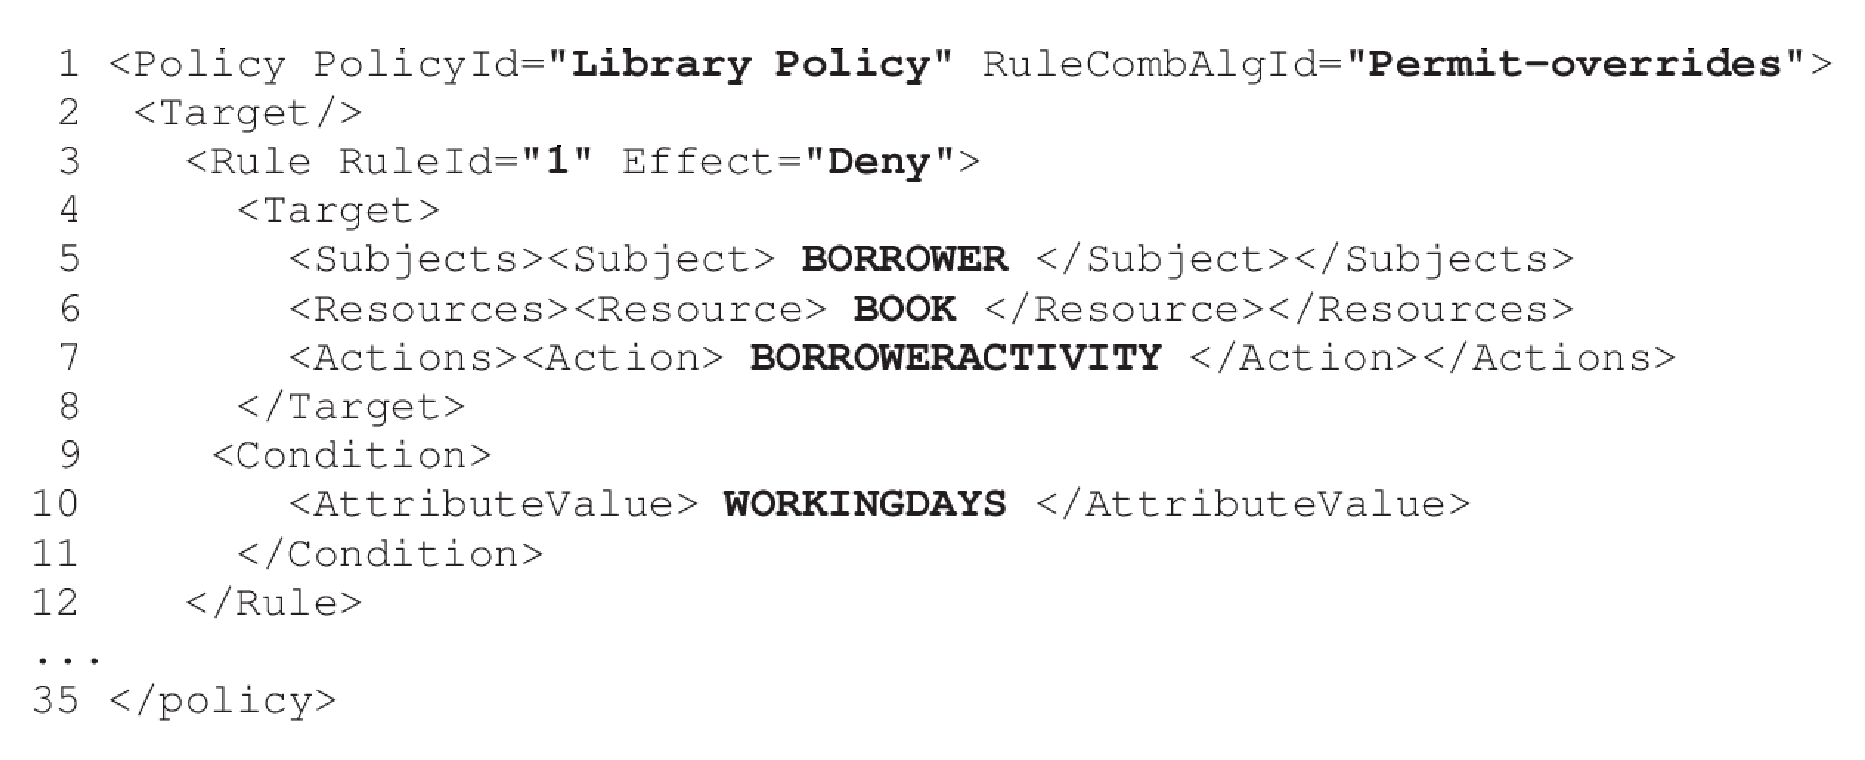
\includegraphics[width=3.5in]{example_mutant.eps}
        \vspace{-5pt}
    \caption{\label{fig:rdcexample}An example mutant policy by changing $R1$'s rule decision (i.e., effect)}
    \vspace{-10pt}
%    \vspace{+3pt}
\end{figure}

%\begin{figure*}[t]%{t}
%\begin{CodeOut}
%\begin{alltt}
% 1 <Policy PolicyId="\textbf{Library Policy}" RuleCombAlgId="\textbf{Permit-overrides}">
% 2  <Target/>
% 3    <Rule RuleId="\textbf{1}" Effect="\textbf{Deny}">
% 4      <Target>
% 5        <Subjects><Subject> \textbf{BORROWER} </Subject></Subjects>
% 6        <Resources><Resource> \textbf{BOOK} </Resource></Resources>
% 7        <Actions><Action> \textbf{BORROWERACTIVITY} </Action></Actions>
% 8      </Target>
% 9	    <Condition>
%10        <AttributeValue> \textbf{WORKINGDAYS} </AttributeValue>
%11      </Condition>
%12    </Rule>
%...
%35 </policy>
%\end{alltt}
%\end{CodeOut}
%\vspace*{-3.0ex} \caption{An example mutant policy by changing $R1$'s rule decision (i.e., effect)}
% \label{fig:rdcexample}
%\end{figure*}


\begin{algorithmic}
\begin{algorithm}[t]
\caption{\label{alg:mutationanalysis}Test Selection based on Mutation Analysis Algorithm}
\STATE{\textit{TestSelection1}($P$, $P_{m}$, $T$): $T'$}
\STATE \textbf{Input:} XACML Policy $P$, modified policy $P_{m}$, Initial Test Cases $T$
\STATE \textbf{Output:} $T' \subseteq T$ where $T'$ is the subset of $T$ selected for use in regression testing $P_{m}$
\STATE {$T'$=\O{}}
\STATE /*Rule-test set-up phase*/
\FOR {each rule $r_{i}$ in Policy $P$}
\STATE {$T_{r_{i}}$=\O{}} where $T_{r_{i}} \subseteq T$ are the tests correlated to $r_{i}$ 
\STATE {/*We mutate the policy $P$ by creating a rule-decision change (RDC) on $r_{i}$ to get $P_{r_{i}}$*/}
\STATE {$P_{r_{i}} \xleftarrow[RDC(r_{i})]{} P$}
\STATE {Execute $T$ with $P_{r_{i}}$}
\FOR {each $t$ in $T$}
\STATE Let $E(t)$ be the test execution result, $E(t)={Success, Failure}$
\IF{$E(t) \leftarrow$ Failure} 
\STATE $T_{r_{i}} \leftarrow T_{r_{i}} \cup t$
\ENDIF
\ENDFOR
\STATE Map($r_{i}$,$T_{r_{i}}$)
\ENDFOR
\STATE /*Test selection phase*/
\STATE $\{r_{m}\}_{i=1..m} \leftarrow diff(P,P_{m})$
\FOR {Each rule $r_{i}$ in $\{r_{m}\}_{i=1..m}$}
\STATE {$T' \leftarrow T' \cup T_{r_{i}}$}
\ENDFOR
\STATE return $T'$
\end{algorithm}
\end{algorithmic}

\subsection{Test Selection based on Mutation Analysis}
Our first proposed test selection technique uses mutation analysis to select test cases as follows. 
The technique needs a preliminary step which is necessary to establish a rule-test correlation.
We next describe rule-test correlation and test selection steps.

\textbf{Rule-Test Correlation Setup.} Given a policy $P$, we create its rule-decision-change (RDC) mutant policy $Pr_i$ by changing decision (e.g., Permit to Deny) of each rule $r_i$ in $P$ in turn.
An example of a mutated policy is shown in Figure~\ref{fig:rdcexample}. In this policy, 
original Rule 1's decision Permit is changed to Deny. The technique finds affected test cases for this rule decision change. 
We execute test cases $T$ on program for $P$ and $Pr_i$. To detect changed policy behaviors, 
the technique monitors responses of evaluated requests formulated from test cases $T$. The test cases, which evaluate different 
policy decisions against $P$ and $P'$, enable to map rule $r_i$ to test cases $t \in T$. The preliminary step ends by establishing 
a correlation between each rule in $P$ and corresponding tests $t \in T$ that trigger this rule.

\textbf{Test Selection.} 
The selection of test cases for regression testing on $P$ and its modified policy $P_m$ starts by conducting change impact analysis 
of $P$ and $P_m$ to find which rules' decision are changed. 
Once these rules are identified, we use the mapping established in the preliminary step to select the subset of 
test cases which are correlated with changed rules.

Algorithm~\ref{alg:mutationanalysis} describes our algorithm used for the technique.
While the technique can quickly select test cases, the technique requires rule-test correlation setup 
(in the preliminary step), which could be costly in terms of execution time. Given n rules in $P$, we execute $T$ for 2$\times$n times. 
As the preliminary step is applied for only existing rules $R$ in $P$, our technique requires addition of rule-test
correlation for newly added rules $R_n$ where $R_n$ $\notin$ $R$ in $P_m$. 
In addition, if a new system test is introduced, we execute this test for 2$\times$n times.
However, an important benefit is that we are enabled to conduct rule-test set-up once before encountering policy 
changes in terms of correlated rules. 


\subsection{Test Selection based on Coverage Analysis}
Our previous technique finds correlation of all of existing rules $N$ in a given policy with the test cases. To reduce
such correlation setup efforts, we develop a technique to correlate only rules, which can be evaluated (i.e., covered)
by test cases. Our intuition is that test cases may interact only with a small number of rules in a policy
instead of all the rules in the policy. We next describe rule-test correlation step.
%We do not describe test selection step, which is identical to the preceding technique.


\begin{algorithmic}
\begin{algorithm}[t]
\caption{\label{alg:coverageanalysis}Test Selection based on Coverage Analysis Algorithm}
\STATE{\textit{TestSelection2}($P$, $P_{m}$, $T$): $T'$}
\STATE \textbf{Input:} XACML Policy $P$, modified policy $P_{m}$, Initial Test Cases $T$
\STATE \textbf{Output:} $T' \subseteq T$ where $T'$ is the subset of $T$ selected for use in regression testing $P_{m}$
\STATE {$T'$=\O{}}
\STATE /*Rule-test set-up phase*/
\FOR {Each test case $t$ in $T$}
\STATE {Execute $t$ with $P$}
\STATE $MAP$=Map($t$,$\{r_{p}\}_{i=1..p}$) where $\{r_{p}\}_{i=1..p}$ are the rules in $P$ that are evaluated (i.e., covered) by $t$
\ENDFOR
%\STATE Generate a mapping rule/test from $MAP_{1}$
%\STATE $MAP_{2}$=Map($r_{i}$,$T_{r_{i}}) \leftarrow MAP_{1}$
\STATE /*Test selection phase*/
\STATE $\{r_{m}\}_{i=1..m} \leftarrow diff(P,P_{m})$
\FOR {Each rule $r_{i}$ in $\{r_{m}\}_{i=1..m}$}
\STATE {$T' \leftarrow T' \cup T_{r_{i}}$}
\ENDFOR
\STATE return $T'$
\end{algorithm}
\end{algorithmic}

\textbf{Rule-Test Correlation Setup.} Given a policy $P$,
Thus we execute test cases $T$ on program that interacts with $P$. Our technique monitors which rules in a policy are evaluated with
requests formulated from test cases $T$. Then, we establish correlation between test cases and evaluated (i.e., covered) rules in $P$. 

%\textbf{Test Selection.} 
%The selection of test cases for regression on $P$ and its modified policy $P_m$ starts by conducting change impact analysis 
%of $P$ and $P_m$ to find which rules' decision are changed. 
%Once these rules are identified, we use the mapping established in the preliminary step to select the subset of 
%test cases which are correlated with changed rules.
\textbf{Test Selection.}
Once the mapping test-rule is established, we proceed test selection step described in the first approach with
the results of change impact analysis of $P$ and $P_m$. The results include information to show which rules' decision have changed.
This test selection maps test cases with those rules to constitute the subset of existing test cases.

Algorithm~\ref{alg:coverageanalysis} describes our algorithm used for the technique.
An important benefit of this technique is to reduce cost in terms of mutation analysis and execution time. This technique does not 
require generating mutants by changing rule's decision in turn. Moreover, the technique can significantly reduce execution time.
While the technique can quickly select system tests in the second step, the technique requires rule-test correlation setup (in the preliminary step), 
which could be costly in terms of execution time. Consider that requests $Rs$ are formulated from test cases interact 
only n$_1$ rules (n$_1$ $\leq$ n) in a policy.
We execute $T$ only once. Our technique requires addition of rule-test
correlation for newly added rules $R_n$ where $R_n$ $\notin$ $R$ in $P_m$ as the same with the previous technique.


\begin{algorithmic}
\begin{algorithm}[t]
\caption{\label{alg:reqevaluation}Test Selection based on Recorded Request Evaluation}
\STATE{\textit{TestSelection3}($P$, $P_{m}$, $T$): $T'$}
\STATE \textbf{Input:} XACML Policy $P$, modified policy $P_{m}$, Initial Test Cases $T$
\STATE \textbf{Output:} $T' \subseteq T$ where $T'$ is the subset of $T$ selected for use in regression testing $P_{m}$
\STATE {$T'$=\O{}}
\STATE {$R_{T'}$=\O{}} where $R_{T'}$ are the requests corresponding to $T'$ 
\STATE {Execute system requests $R$}
\FOR {each request $Re$ in $R$}
\IF {$decision(Re/_{P}) \neq decision(Re/_{P_{m})}$}
\STATE {$R_{T'} \leftarrow R_{T'} \cup Re$}
\ENDIF
\ENDFOR
\STATE {$T' \leftarrow R_{T'}$}
\STATE return $T'$
\end{algorithm}
\end{algorithmic}

\subsection{Test Selection based on Recorded Request Evaluation}
To reduce such correlation setup efforts in the previous techniques, we develop
a technique, which does not require rule-test correlation setup.
Instead of correlation, our technique records test cases and their issued requests as a preliminary step.
More specifically, our technique executes test cases $T$ on a program for $P$ and records all requests issued to policy decision point (PDP) for each test case. For test selection, our technique evaluates all issued requests against $P$ and $P_m$ and selects the test subset of
requests (with corresponding system test cases) that engender different decisions for two different policy versions.

%While our previous two techniques require correlation rule-test setup. 
%The techniques analyze two versions of policies statically 
%or dynamically under test to find which rules' are changed. However, these technique require correlation setup.
Algorithm~\ref{alg:reqevaluation} describes our algorithm used for the technique.
The current approach requires the execution of system test cases $T$ only once.
% For additional test cases, we execute the tests only once. 
Moreover, while the two previous techniques are white-box testing since access control policies are available, the present technique 
does not require the availability of access control policies. This can present a considerable advantage when developers don't want 
to reveal their access control policies.



\subsection{Test Augmentation}
\label{subsec:testaugmentation}
While test-selection techniques are useful for selecting test cases for a program impacted by policy changes, these test cases may not sufficiently cover all the rules in the policy impacted by the changes.
We develop a test augmentation technique, which complements our test-selection techniques by generating additional test cases to 
cover not-covered-impacted-rules $N_r$ by existing test cases.

Our augmentation technique first analyzes change impact analysis between $P$ and $P'$ to find rules impacted by policy changes.
The technique finds $N_r$ by evaluating selected test cases and monitoring which 
rules are evaluated during test case execution.
%our selected test cases and $P$ and $P'$. 
For $N_r$, we next generate requests, which can cover $N_r$.
We then analyze existing test cases to create test cases, which issue the requests
to cover $N_r$ with minimal changes in test cases.
For example, attribute change (e.g., subject element change from $Student$ to $Professor$) may cover $N_r$. We then verify that augmented test cases increase coverage of $N_r$.
%[TBD]

%\textbf{Distance-based complexity: Besides the simple graph 
%complexity, we extract distance-based complexity measures 
%based on the shortest distance between all pairs of crash 
%graph nodes using the Floyd-Warshalls algorithm  [7]. The 
%initial distance between two connected nodes is set to 1. 
%Then, we compute distance-based complexities such as 
%eccentricity, density and radius. For example, the eccentricity 
%of a node v is the greatest distance between v and any other 
%node. We aggregate all eccentricities with minimum 
%(=radius), maximum (=diameter) and average. Table III 
%describes selected features, while detailed measures are 
%described in [21].}










\section{Implementation} \label{sec:implementation}

Our implementation (written in Java) includes five components: regression simulator, test-rule correlation, request-record, test selection,
and test augmentation. To simulate regression in access control policies, 
we used three types of mutants injected in the policies; RMR (Rule Removal), RA (Rule Addition), and RDC (Rule Decision Change)
mutants. The regression simulator analyzes a policy and injects one
of such changes. For RMR, given a randomly selected rule in a policy $P$,
the regression simulator removes the rule. For RDC, given a randomly selected rule in a policy $P$, the regression simulator changes
the decision of the rule. For $RA$, the regression simulator adds a randomly generated rule with random attributes collected from $P$ in a random place.
The simulator can inject more than one type of changes to $P$ for simulating regression on $P$.

For test selection based on mutation analysis technique,
our test test-rule correlation mutates a given policy using RDC, executes all of test cases for each mutated policy, and monitors changed
behaviors by comparing test results of the test cases with an original policy or its mutated policy.
The component also automatically compares the testing results (on the policy and the mutated policies) and logs killed mutant information if the results are inconsistent. We use
such killed mutant information for rule-test correlation.
For test selection based on coverage analysis technique, we execute all of test cases once and monitors
which rules are evaluated for each test case execution. We use such coverage information for rule-test correlation.
For the test selection based on recorded request evaluation,
the request-record component records all requests issued by test cases and evaluated rules in a policy.

For our first two techniques, the test selection component requires change impact analysis to
show changed policy behaviors of two versions of policies.
The implementation leverages an existing access control policy verification tool called Margrave~\cite{fisler05:verification}. 
Margrave is a tool suite for analyzing access control policies written in XACML.
Given two versions of policies, $P$ and $P'$, 
our implementation uses the generic APIs of Margrave to
print out all the policy changes with their corresponding changed decisions in a summarized format.
Our first two techniques analyze the results of Margrave and
find which rules $R_i$ impacted by policy changes. We then find all of test cases $R_t$
impacted by $R_i$.

For the test selection based on recorded request evaluation,
the component does not require change impact analysis. The test selection
component log recorded requests to reveal different evaluated decision against $P$ and $P'$.

The test argumentation component compares
not-covered policy behaviors $r_1$s (i.e., represented by requests) with requests $r_2$s
issued from existing test cases. The test argumentation computes
similarity between $r_1$ and $r_2$ to decide applicability of modification for test
argumentation. Given recommended test cases with high similarity score,
we manually modify the test cased to cover not-covered policy behaviors. 
If not applicable for modification, the component
generates a test cases to issue such requests to cover not-covered policy behaviors. 




\section{Experiment}\label{sec:experiment}

We carried out our evaluation on a desktop PC, running Windows 7 with Intel Core i5, 2410 Mhz processor, and 4 GB of RAM. 
We have implemented test selection techniques and mutant generation in Java.
We generate mutants by changing rules
in access control policies To simulate regression in access control policies.
We used three types of mutants injected in the policies; the first one
is RMR (Rule Removal), RA (Rule Addition), and CRE (Change Rule Effect)
mutants. [ToDo: citation and explain more] In our mutants, we only change rules in access control policies,
we do not simulate regression in test code in subjects.
To measure the efficiency of our three techniques, we conducted evaluation as follows. 
We compared elapsed time to analyze test-rule correlation analysis,
change impact analysis, and test selection by each technique.
For the first two techniques, we require test-rule correlation analysis
and change impact analysis, which should be done before actual test selection.
We compare also selected tests by our three techniques to
compare that all of these techniques return the same tests for regression.
The objective of this evaluation is to investigate how our approach impacts performance for subjects and safety
to select all tests for regression.


%\textbf{Detection: -- selection detection two Type} evaluated result inconsistency and number of reqs (in case of dependency) or failure trace info
  

\begin{table*}[tbp]
  \centering
  	\caption{Subjects}    
    \begin{tabular}{|l|r|r|r|r|r|r|}
    \hline
          & LOC   & \# of Test Methods & \# of Security Test Methods & \# of Covered Rules & \# of Not-covered Rules & \% of Covered Rules \\\hline\hline
    LMS   & 3749  & 46    & 29    & 42    & 0     & 100 \\\hline
    VMS   & 3734  & 52    & 10    & 13    & 106   & 12 \\\hline
    ASMS  & 7836  & 93    & 91    & 109   & 21    & 83 \\\hline
		\end{tabular}%
  \label{tab:subj}%
%\end{table}%
%
%\begin{table*}[tbp]
  \centering
  \caption{Access control policies in our subjects}
    \begin{tabular}{|l|r|r|r|r|r|r|r|}
 		\hline
     & ~\# Subjects~ & ~\# Actions~ & ~\# Resources~ & ~\# Conditions~ & ~\# Explicit Rules~ & ~\# Implicit Rules~ & ~\# Total Rules~ \\\hline\hline
    LMS   & 6     & 10    & 3     & 4     & 42    & 678   & 720 \\\hline
    VMS   & 7     & 15    & 3     & 3     & 106   & 839   & 945 \\\hline
    ASMS~  & 8     & 11    & 5     & 4     & 129   & 1631  & 1760 \\\hline
 
    \end{tabular}%
  \label{tab:subjectpolicies}%
\end{table*}%

\subsection{Subjects}
The subjects include three real-life Java programs each which
interact with access control policies \cite{testcase}. We next describe
our three subjects.
\begin{itemize}	
\item Library Management System (LMS) provides web services to manage books in a public library.
\item Virtual Meeting System (VMS) provides web conference services. VMS allows users to organize
online meetings in a distributed platform.
\item Auction Sale Management System (ASMS) allows users to buy or sell items on line. A seller initiates an auction by submitting a description of an item she wants to sell with its expected minimum price. Users then participate in bidding process by
bidding the item. For the bidding on the item, users have enough money in her account before bidding.
\end{itemize}

Table~\ref{tab:subj} shows information in our subjects. [ToDo: explain more]
Table~\ref{tab:subjectpolicies} shows information in our subjects. [ToDo: explain more]
Our subjects are equipped with Sun PDP \cite{sunxacml}, which is
a popularly used PDP to evaluate requests.
Policies in LMS,VMS, and ASMS contain a total of 720, 945, and 1760 rules, respectively.
%Moreover, to compare performance improvement over existing PDPs,
%we adopt XEngine (instead of Sun PDP) in our subjects to evaluate requests.
%XEngine is a novel policy evaluation engine, which transforms the hierarchical tree structure of the XACML policy to a flat structure
%to improve request processing time. XEngine also handles various combining algorithms supported by XACML.
 


\subsection{Objectives and Measures}
In the evaluation, we intend to answer the following
research questions:
\begin{itemize}


	\item RQ1: How many of test cases in a test suite (from an existing test suite) selected by our test selection techniques? This question helps to show that our techniques can reuse ZZ\% of a test suite. We also compare our approach with random test select technique to show how effectively our approach selects test suite to cover changed policy behaviors.
	
	\item RQ2: Do our protest selections are safe? This question helps to show that our techniques select all tests, which shows only and all test cases to reveal changed behaviors in access control policies.
	
	\item RQ3: What are elapsed time for our techniques to conduct test selection by given subjects? This question helps to compare performance of our techniques by measuring
	efficiency with regards to elapsed time.
			
	\item RQ4: How higher we can achieve additional policy coverage ratio by our test augmentation technique?  This question helps to show that our technique can generate/augment test suite to cover 100\% of changed policy behaviors. We also compare our approach with random test generation technique to show how effectively our approach augment test suite to cover not-coverted changed policy beahviors.
			
%	How many of test cases in a test suite (from an existing test suite) selected by our test selection technique? This question helps to show that our technique can reuse number of a test suite. We also compare our approach with random test select technique to show how effectively our approach selects test suite to cover M.
%RQ1: How many of test cases in a test suite (from an existing test suite) selected by our test selection technique? This question helps to show that our technique can reuse __ % of a test suite. We also compare our approach with random test select technique to show how effectively our approach selects test suite to cover M.
%RQ2: How higher we can achieve additional policy coverage ratio by our test augmentation technique?  This question helps to show that our technique can generate/augment test suite to cover 100\% of M. We also compare our approach with random test generation technique to show how effectively our approach augment test suite to cover M.

%	\item RQ4: Safe? compare three ones or compare all of test cases to find whether it was complete and safe?
%	
%	\item RQ2: Performance Comparision of these three ones?
%	
%	\item RQ3: How higher we can achieve additional policy coverage ratio by our test augmentation technique?  This question helps to show that our technique can generate/augment test suite to cover 100\% of M. We also compare our approach with random test generation technique to show how effectively our approach augment test suite to cover M.
	
\end{itemize}

\subsection{Metrics}

We use following 4 metrics in our evaluation.
\begin{itemize}
	\item Policy coverage information for changed policy behaviors.
	\item Number of test cases reused by the test selection technique.
	\item Elapsed time of test-rule correlation, change impact analysis, and test selection.
	\item Number of test cases generated by the test augmentation technique. 
\end{itemize}
	
[ToDo: explain more]

% Table generated by Excel2LaTeX from sheet 'Sheet1'


%Metrics # of code
%Metrics # of rules in a policy
%Metrics # of system tests
%	seucrity tests
%	selected tests


%In our evaluation, we measure request processing time by evaluating randomly
%generated requests developed by our previous work~\cite{Xengine}.
%In particular, for multiple PDPs, our approach fetches a PEP with a corresponding
%PDP for a given request at run time. Therefore, request processing time includes
%both fetching time and request evaluation time.


%\begin{figure*}[h!]
%  \centering
%  \subfloat[LMS]{\label{fig:gull}\includegraphics[width=0.33\textwidth]{LMS.pdf}}                
%  \subfloat[VMS]{\label{fig:VMS}\includegraphics[width=0.33\textwidth]{VMS.pdf}}
%  \subfloat[ASMS]{\label{fig:ASMS}\includegraphics[width=0.33\textwidth]{ASMS.pdf}}
%  \caption{Request Processing Time for our subjects LMS, VMS and ASMS}
%  \label{fig:processing time}
%\end{figure*}

%\subsection{Performance Improvement Results}\label{subsec:performanceimprovement}
%
%We generated the resulting sub-policies for all the splitting criteria defined in Section~\ref{subsec:SplittingCriteria}.
%For each splitting criteria, we have conducted systems tests to generate requests that trigger all the PEPs in the evaluation. 
%The test generation step leads to the execution of all combination of possible requests described in our previous work \cite{testcase}.  
%The process of tests generation is repeated for ten times in order to avoid the impact of randomness.
%We applied this process to each splitting criterion and calculated evaluation time on average of a system under tests.

\section{Related Work}
\label{sec:related}


Various techniques have been proposed on regression testing of software programs in software engineering and
programming language communities~\cite{Rothermel:1996:ART:235681.235682, Graves:2001:ESR:367008.367020, cite{Elbaum:2000:PTC:347324.348910,santelices08sep}}.
These techniques aim to select every test case to reveal different behaviors correctly after modification
in program or to augment test cases.
These techniques are related to regression test selection \cite{Rothermel:1996:ART:235681.235682}, 
\cite{Graves:2001:ESR:367008.367020}, test-suite prioritization \cite{Elbaum:2000:PTC:347324.348910}, and test-suite augmentation \cite{santelices08sep}. 
Note that these techniques focus on changes at code level.
None of these techniques consider potential changes that can arise from code-related components (such as a policy that interacts with application code).
Polices and general programs are fundamentally different in terms of structures, semantics, and
functionalities, etc. Therefore, techniques for regression
testing of general programs are not suitable for addressing 
the test selection problem for policy evolution.
Our work is the first one for automatic test-selection approach in context of policy
evolution.

Prior work that is closest to ours is Mouelhi et al. work~\cite{mouelhi09:tranforming}.
They proposed a technique to transform functional test cases into security test cases. 
These test cases are then used to verify correctness of access control mechanisms in policy-based systems.
They defined various mutation operators at the policy level.
Given a policy and its mutated policy, the technique selects only impacted test cases to be transformed as security test cases
(with additional manual task to add code for checking security).
While this work focuses on security test case selection from initial test cases,
our work focuses on test selection problem impacted by policy changes
to reveal faults induced by policy changes.

Another work closest to ours is Fisler et al.'s
work~\cite{Fisler:2005:VCA:1062455.1062502}.
They developed a tool called ``Margrave'' that enables verifying properties against 
policies written in XACML and conducting change impact analysis. Margrave is based on multi-terminal binary decision diagrams and allows several forms of 
constraints to be added as properties in the Scheme programming language.
While Margrave is effective to detect changed policy behaviors between two versions
of a policy specified in XACML at policy level, Margrave does not handle with situations where
program behaviors are changed by policy changes as our work focuses on.

%in terms of regression testing. As application
%code can often interact with policies, our work is useful

To facilitate verifying and validating the correctness of policies, prior
research work has been done in the area of policy testing, which generates and executes test cases against a policy.
Martin et al.~\cite{martin06:defining} proposed a framework to detect policies faults by analyzing
policy test suites that involve 
requests-responses pairs. The framework is based on mutation operators~\cite{martin07:fault} that enable measuring fault detection capability. 
It uses a tool~\cite {martin07:automated} that aims at minimizing the test cases to be generated by analyzing the structural coverage of the policies.
Hu et al.~\cite{hu07:conformance} proposed a generic model-based conformance checking technique for access control policies written in
XACML.
These approaches focus on test request generation at a policy level (e.g., policies written in XACML).
Instead of generating new requests, our work focuses on regression testing at the implementation level (the system level) by
reusing existing hardcoded test cases.
%, which includes
%application code when a policy evolves. 


%Margrave detects the presence of requests that may violate the specified properties.

%used these mutated policies to select impacted tests. The impacted tests are then tranformed to security tests (by added specific code to check the security mechanism). 
%Although this work focused on applications interacting with policies, it was not presented from a regression testing perspective.
%
%
%The most relevant paper that is related to our work was presented by Mouelhi et al. in~\cite{mouelhi09:tranforming}. The authors proposed transforming functional tests into security tests. 
%These tests can then be used to validate the access control mechanisms in policy-based systems. They defined mutation operators at the policy level and used these mutated policies to select impacted tests. The impacted tests are then tranformed to security tests (by added specific code to check the security mechanism). 
%Although this work focused on applications interacting with policies, it was not presented from a regression testing perspective. 

%fault
%localization problem of ?rewall policies.
%
%This paper focuses on regression testing for policy-based software systems.

 


%Zhang et al \cite{DBLP:conf/isw/ZhangRG05} used model checking technique which is supported by a tool to evaluate access
%control policies specified in a modelling formalism called RW. Hughes et al. \cite{hughes04:automated} proposed using First-Order Logic 
%to automatically verify access control policies. Their model is based on specifying access to resources, they show that the access
%control policies in XACML can be translated into a normlized form that includes four classes: permit,
%deny, error, and not-applicable. A partial ordering among access control polices enable the authors to specify properties that are checked later
%with Alloy analyszer \cite{Alloy}. Nyanchama et. al. \cite{Nyanchama99therole} focused on policy analysis and verification related to 
%RBAC models. They used graphs to model hierarchies of users, roles and permissions and to solve role-role conflicts issues.
%While these different approaches focus on test request generation for validating the policy implementation (the XACML code), 
%the technique presented in this paper focuses on regression testing at the implementation level (the system level) which occurs when the access control policy evolves. 





\Comment{
Our previous work~\cite{hu10:model,hu08:property} presented
model checking to verify various policies such as role-based
access control policies~\cite{ferraiolo92:role}.
Our previous work translates policies into specifications
in NuSMV~\cite{cimatti02:nusmv2}. NuSMV verifies the specifications against properties. 
Based on our previous work, we developed a tool, called ACPT\footnote{http://csrc.nist.gov/groups/SNS/acpt/index.html},
to verify and test access control policies.
However, our previous work does not detect conflicts
or redundancies between two policies, one major
focus of our current work. Moreover, our previous
work does not recommend any combinations (to the policy
authors) that can be recommended by our current work. 

There exist tools to verify XACML policies. These tools require XACML policies in formal specification languages such as 
Alloy~\cite{jackson01:micromodularity}. Hughes et al.~\cite{hughes04:automated} proposed an approach to translate XACML policies to a model 
specified in the Alloy language~\cite{jackson01:micromodularity}. Then, the Alloy Analyzer verifies whether the model satisfies the given properties.
Kolovski et al.~\cite{kolovski07:analyzing} converted XACML policies into specifications in  description logics (DL) and adopted existing DL 
verification tools to verify the specifications. Fisler et al.~\cite{fisler05:verification} developed a Binding Decision Diagram (BDD) based 
verification tool, called Margrave, to verify XACML policies. Margrave parses XACML policies into the BDD structure. Moreover, Margrave supports 
change-impact analysis to report which decisions are changed after policy modification.
Similar to these previous approaches, our approach focuses on modeling and verifying policies via a symbolic model checking. Moreover, our approach
 verifies whether two policies may include conflicts and redundancies via a symbolic model checking. 
While these previous approaches do not help combining two policies, our approach recommends combinations of two policies that could satisfy 
user-specified properties. 


%\textbf{Policy Combinations/Integration.}
%Bonatti et al.~\cite{Bonatti2} proposed combining sub-policies based on 2-valued algebra. 
Backes et al.~\cite{backes04algebra} proposed a 3-valued algebra to combine sub-policies considering privacy policies.
 They defined relations of combination with three operators: conjunction, disjunction, and scoping.
 Li at el.~\cite{Ninghui2009} proposed an algebra for combining sub-policies. 
They introduced new combining algorithms such as weak majority or strong majority.
For example, in the case of the strong majority combining algorithms, at least 2/3 
rules evaluated against a request should be evaluated to the same decision. Since the decision is the majority, 
the decision is returned as a final decision. They proposed algebras to generalize their combining algorithms.
%Mazzoleni et al.~\cite{Mazzoleni2006} proposed policy integration that can be applied to XACML policies. 
In their approach, policy authors can specify conditions to represent how their policies can be integrated with other policies. 
Their integration approach is based on analysis of two policies to be integrated. Policy authors measure similarity of two policies 
and integrate the policies based on given condition.





}
\Comment{
%\textbf{Policy Change Impact Analysis}
%\textbf{Policy Conflict and Redundancy}
%\textbf{Verification in NuSMV for other projects}

%interaction, but runtime ...more general stuff to do it.

\textbf{Policy Verification.}
There are verification tools available for XACML
policies. Hughes et
al.~\cite{hughes04:automated}
proposed an approach
to verify XACML policies by
translating the policies to the Alloy
language~\cite{jackson01:micromodularity}.
Then, they use Alloy Analyze to verify properties
against the translated policies. 
Zhang et
al.~\cite{zhang05:evaluating} developed a model-checking tool
to verify policies specified in
\Intro{RW} languages~\cite{zhang04:synthesis}, which can be converted to
XACML.
Kolovski et
al.~\cite{kolovski07:analyzing} formalize XACML policies with
description logics (DL), which are a decidable fragment of
first-order logic, and exploit existing DL verifiers to conduct
policy verification.
Schaad and Moffett~\cite{schaad02:lightweight} leverage
Alloy~\cite{jackson01:micromodularity} to check that role-based
access-control policies do not allow roles to be assigned to users
in ways that violate SoD constraints.
Similar to previous research work, our work also model and verify policies
via model checking. However, we extend
our work to detect conflict and redundancy via a symbolic checker.


\textbf{Policy Combinations/Integration.}
Bonatti et al.~\cite{Bonatti2} proposed combining sub-policies based on 2-valued algebra. Backes et al.~\cite{backes04algebra} proposed a 3-valued algebra to combine sub-policies considering privacy policies. They defined relations of combination with three operators: conjunction, disjunction, and scoping. Li at el.~\cite{Ninghui2009} proposed an algebra for combining sub-policies. They also introduce new combining algorithms such as weak majority or strong majority. For example, in case of the strong majority combining algorithms, at least 2/3 rules evaluated against a request should return the same decision. As the decision is majority, the decision is returned as a final decision. They propose algebras to generalize their combining algorithms. Moreover, they propose combinations of sub-policies, which may return policy evaluation errors and obligations.
Mazzoleni et al.~\cite{Mazzoleni2006} proposed policy integration that can be applied to XACML policies. In their approach, policy authors can specify conditions to represent how their policies can be integrated with other policies. Their integration approach is based on analysis of two policies to be integrated. Policy authors measure similarity of two policies and integrate the policies based on given condition.
We also propose that a methodology to combine two policies using property verification.
We next describe a methodology to recommend the combinations (of two policies) that could satisfy user-specified properties.

\textbf{Policy Testing.}

Our previous work~\cite{hu10:model} demonstrated an approach
to represent a policy and its properties as
corresponding finite state machine (FSM) model and temporal
logics (e.g., computation tree logic), respectively, using SMV specification language~\cite{cimatti02:nusmv2}.

Our previous work developed policy testing approaches for policy
structural coverage~\cite{martin06:defining}, request
generation~\cite{martin07:automated}, and mutation
testing~\cite{martin07:fault}.
% Our previous
%work~\cite{hu07:conformance} also proposed a generic model-based
%conformance checking approach for access control policies written in
%XACML.
These pieces of work do not rely on properties for generating
test requests to detect a fault in a policy. 
Our previous work~\cite{martin08:assessing} developed an approach
for measuring the quality of policy properties in policy
verification. Given user user-specified
properties, the quality of properties are measured
based on fault-detection capability.
}
\section{Conclusion}
\label{sec:conclusion}

We make three key contributions in this paper. First, we proposed three test selection techniques for access control policy evolution. 
To the best of our knowledge, our paper is the first one for automatic test-selection approach in context of policy
evolution. Second, we presented a test augmentation technique to generate test cases that cover not-covered
policy changes by existing test cases. Third, we conduct evaluation with few test metrics to measure the effectiveness of our approach and the efficiency of our three test selection
techniques.
The evaluation results demonstrated that our approach is effective to select test cases for test reduction.
Among the proposed three test-selection techniques, the evaluation results demonstrated that the technique based recorded
request evaluation is the most efficient compared with the first two techniques. Besides, we also achieve 100\% coverage
of changed policy behaviors with augmented test cases.

%
%generate additional new test cases to cover not-covered-impacted-rules with selected test cases by the preceding techniques.
%
%to select every test case impacted by policy changes.
%
%
%from existing test cases to test program code impacted by policy changes.
%
%comprehensive fault model for ?rewall
%policies, including ?ve types of faults. For each type of
%fault, we present an automatic correction technique. Second, we propose the systematic approach that can automatically correct all or part of the misclassi?ed packets
%of a faulty ?rewall policy. To the best of our knowledge,
%our paper is the ?rst one for automatic correction of ?rewall policy faults. Last, we implemented our approach
%and evaluated its effectiveness on real-life ?rewalls. To
%measure the effectiveness of our approach, we propose
%two metrics, which we believe are general metrics for
%measuring the effectiveness of ?rewall policy correction
%tools. The experimental results demonstrated that our approach is effective to correct a faulty ?rewall policy with
%three types of faults:
%
%Conclusion here!!


%ACKNOWLEDGMENTS are optional
%\section{Acknowledgments}
%This section is optional; it is a location for you
%to acknowledge grants, funding, editing assistance and
%what have you.  In the present case, for example, the
%authors would like to thank Gerald Murray of ACM for
%his help in codifying this \textit{Author's Guide}
%and the \textbf{.cls} and \textbf{.tex} files that it describes.

%
% The following two commands are all you need in the
% initial runs of your .tex file to
% produce the bibliography for the citations in your paper.
\bibliographystyle{abbrv}
\bibliography{yangtse,yangtse2}  % sigproc.bib is the name of the Bibliography in this case
% You must have a proper ".bib" file
%  and remember to run:
% latex bibtex latex latex
% to resolve all references
%
% ACM needs 'a single self-contained file'!
%
%APPENDICES are optional
%\balancecolumns
%\appendix
%%Appendix A
%\section{Headings in Appendices}
%The rules about hierarchical headings discussed above for
%the body of the article are different in the appendices.
%In the \textbf{appendix} environment, the command
%\textbf{section} is used to
%indicate the start of each Appendix, with alphabetic order
%designation (i.e. the first is A, the second B, etc.) and
%a title (if you include one).  So, if you need
%hierarchical structure
%\textit{within} an Appendix, start with \textbf{subsection} as the
%highest level. Here is an outline of the body of this
%document in Appendix-appropriate form:
%\subsection{Introduction}
%\subsection{The Body of the Paper}
%\subsubsection{Type Changes and  Special Characters}
%\subsubsection{Math Equations}
%\paragraph{Inline (In-text) Equations}
%\paragraph{Display Equations}
%\subsubsection{Citations}
%\subsubsection{Tables}
%\subsubsection{Figures}
%\subsubsection{Theorem-like Constructs}
%\subsubsection*{A Caveat for the \TeX\ Expert}
%\subsection{Conclusions}
%\subsection{Acknowledgments}
%\subsection{Additional Authors}
%This section is inserted by \LaTeX; you do not insert it.
%You just add the names and information in the
%\texttt{{\char'134}additionalauthors} command at the start
%of the document.
%\subsection{References}
%Generated by bibtex from your ~.bib file.  Run latex,
%then bibtex, then latex twice (to resolve references)
%to create the ~.bbl file.  Insert that ~.bbl file into
%the .tex source file and comment out
%the command \texttt{{\char'134}thebibliography}.
%% This next section command marks the start of
%% Appendix B, and does not continue the present hierarchy
%\section{More Help for the Hardy}
%The acm\_proc\_article-sp document class file itself is chock-full of succinct
%and helpful comments.  If you consider yourself a moderately
%experienced to expert user of \LaTeX, you may find reading
%it useful but please remember not to change it.
\balancecolumns
% That's all folks!
\end{document}
